\documentclass[
a4paper, 12pt, % Papierformat, Schriftgröße
titlepage, 		 % extra Titelseite statt einfacher Überschrift
twoside,			 % beidseitiger Druck
headsepline,	 % Trennlinie für die Kopfzeile
BCOR5mm,			 % Binderand 5 mm
idxtotoc, bibtotoc]{scrreprt}	% Index (soweit vorhanden) und Literaturliste 
				       % im Inhaltsverzeichnis aufführen
% Dokumentenklasse ist aus dem KOMA-Script-Paket die SCRReprt-Klasse.

\usepackage{wsi-ra}

% Eigene Pakete
\usepackage{siunitx}

\usepackage{tikz}
\usetikzlibrary{arrows,automata,positioning,matrix,fit}
\usepackage{tikz-uml}

\usepackage{pgfplots}
\usepackage{booktabs}
\pgfplotsset{compat = newest}

\newcommand*{\captionsource}[2]{%
  \caption[{#1}]{#1 Quelle: #2}}

\usepackage[T1]{fontenc}
% JSON stuff
%\usepackage{bera}% optional: just to have a nice mono-spaced font
\usepackage{listings}
\usepackage{xcolor}
\colorlet{punct}{red!60!black}
\definecolor{background}{HTML}{EEEEEE}
\definecolor{delim}{RGB}{20,105,176}
\colorlet{numb}{magenta!60!black}
\lstdefinelanguage{json}{
    basicstyle=\normalfont\ttfamily,
    numbers=left,
    numberstyle=\scriptsize,
    stepnumber=1,
    numbersep=8pt,
    showstringspaces=false,
    breaklines=true,
    frame=lines,
    backgroundcolor=\color{background},
    literate=
     *{0}{{{\color{numb}0}}}{1}
      {1}{{{\color{numb}1}}}{1}
      {2}{{{\color{numb}2}}}{1}
      {3}{{{\color{numb}3}}}{1}
      {4}{{{\color{numb}4}}}{1}
      {5}{{{\color{numb}5}}}{1}
      {6}{{{\color{numb}6}}}{1}
      {7}{{{\color{numb}7}}}{1}
      {8}{{{\color{numb}8}}}{1}
      {9}{{{\color{numb}9}}}{1}
      {:}{{{\color{punct}{:}}}}{1}
      {,}{{{\color{punct}{,}}}}{1}
      {\{}{{{\color{delim}{\{}}}}{1}
      {\}}{{{\color{delim}{\}}}}}{1}
      {[}{{{\color{delim}{[}}}}{1}
      {]}{{{\color{delim}{]}}}}{1},
}
\usepackage{enumitem}
\usepackage{adjustbox}
%\usepackage{tabularx}
\usepackage{makecell}
\usepackage{float}
\usepackage{dirtree}
\usepackage{multicol}
\usepackage{wrapfig}
\usepackage{subcaption}

%%%%%%%%%%%%%%%%%%%%%%%%%%%%%%%%%
% Gestaltung der Titelseite     %
%%%%%%%%%%%%%%%%%%%%%%%%%%%%%%%%%
\titlehead{\vspace{.5cm}\centering
\textbf{\textsc{Eberhard-Karls-Universität Tübingen}}\\
Wilhelm-Schickard-Institut für Informatik\\Lehrstuhl Kognitive Systeme}

\subject{\large Bachelorarbeit Informatik}
% Studien-, Bachelor-, Diplom- oder Masterarbeit

% Der Titel
\title{\begin{tabular}{p{11cm}}\centering\Large
Einsatz von Deep Learning zur Erkennung von Messspitzen in Rasterelektronenmikroskopen
\end{tabular}}

% Der Name des Autors
\author{\large David Stefan Kleindiek}
\date{} % Hier kein Datum eintragen!

% Die Betreuer sowie das Abgabedatum etc.
% Zweitbetreuer: nicht bei Bachelor Informatik. Nur Master sowie Kognitionswissenschaften.
% Zweitbetreuer ist nie der Betreuende Doktorand!
\publishers{\normalsize\centering\begin{tabular}{p{3cm}p{8cm}}
\textbf{Betreuer:} 	& Prof.\,Dr.\,rer.\,nat.~Andreas Zell\\
			& Wilhelm-Schickard-Institut für Informatik\\
      & \\
			& Dr.~Matthias Kemmler\\
			& Kleindiek Nanotechnik GmbH\
      & \\
\textbf{Begonnen am:}	& 1. Juli 2023\\
 			& \\
\textbf{Beendet am:}	& \today
\end{tabular}}


%%%%%%%%%%%%%%%%%%%%%%%%%%%%%%%%%
% Eidesstattliche Erklärung     %
%%%%%%%%%%%%%%%%%%%%%%%%%%%%%%%%%

\uppertitleback{\ \\[4ex]\centering
\begin{tabular}{>{\normalsize}p{4.5cm}>{\normalsize}p{4cm}}
\large\textbf{Erklärung} & \\[4ex] \multicolumn{2}{p{8.5cm}}{\normalsize
Hiermit versichere ich, diese Arbeit selbstständig verfasst und nur die
angegebenen Quellen benutzt zu haben.}\\
\\[2ex]\multicolumn{2}{p{8.5cm}}{\normalsize Tübingen am \today}\\[6ex]
\begin{tabular}{p{4.2cm}}\cline{1-1}\\\end{tabular}&\\
David Stefan Kleindiek
\end{tabular}}
\lowertitleback{} % Hier nichts eintragen!


%%%%%%%%%%%%%%%%%%%%%%%%%%%%%%%%%
% Beginn des Dokumentes         %
%%%%%%%%%%%%%%%%%%%%%%%%%%%%%%%%%

\begin{document}


%%%%%%%%%%%%%%%%%%%%%%%%%%%%%%%%%
% Titelei                       %
%%%%%%%%%%%%%%%%%%%%%%%%%%%%%%%%%

\pagenumbering{roman}		% kleine lateinische Seitenzahlen
\maketitle
\begin{abstract}
\textbf{Kurzfassung. }Die Halbleiterindustrie, eine sich ständig weiterentwickelnde und komplexe Branche, die sich auf Strukturen unter 10 Nanometern reduziert hat, steht vor ständigen Herausforderungen bei der Fehleranalyse der entwickelten Strukturen. Insbesondere die zuverlässige Lokalisierung von Messspitzen im Nanoprobing ist entscheidend, um die Effizienz durch Automatisierung zu steigern und gleichzeitig Beschädigungen zu vermeiden. Diese Bachelorarbeit beschäftigt sich mit der Entwicklung und Implementierung von Deep Learning-Verfahren, insbesondere des Mask R-CNN Modells, zur Detektion von Messspitzen in rasterelektronenmikroskopischen Bildern.

Durch die Entwicklung und Implementierung von Schnittstellen zu Kleindiek Manipulatoren und ZEISS Mikroskopen in Python wird die Datenerfassung automatisiert und ein umfangreicher Datensatz für Nanoprobing erzeugt. Das Modell wird angepasst und trainiert, um die spezifischen Herausforderungen des Bildrauschens und der Formenvielfalt der Messspitzen zu überwinden.

Die Arbeit gibt einen detaillierten Einblick in den Nanoprobing-Prozess, und beinhaltet die umfassende Implementierung, das Training und die Evaluierung des Mask R-CNN Modells. Die Ergebnisse dieser Arbeit deuten darauf hin, dass Deep Learning eine vielversprechende Lösung für die Prozessautomatisierung in der Fehleranalyse in der Halbleiterindustrie ist und bieten eine solide Grundlage für die weitere Automatisierung und Verbesserung der Fehleranalyse, die Modelle zu optimieren und die Technologie in bestehende Prozesse zu integrieren.
\end{abstract}

%\chapter*{Danksagung}
Ich danke allen, die an dieser Arbeit mitgewirkt haben. Eine Danksagung ist
grundsätzlich nicht nötig und darf durchaus entfallen. Falls gewünscht, ist die
Danksagung an dieser Stelle einzufügen.


\tableofcontents		% Inhaltsverzeichnis
%\cleardoublepage		% Erzeugt neue Leerseite. Muss ggf. auskommentiert werden.
\clearpage
\pagenumbering{arabic}		% Ab hier mit arabischen Zahlen numerieren


%%%%%%%%%%%%%%%%%%%%%%%%%%%%%%%%%
% Beginn der eigentlichen Arbeit%
%%%%%%%%%%%%%%%%%%%%%%%%%%%%%%%%%

%\input{tex/01_Einfuehrung_vorlage}
\chapter{Einführung}
\section{Motivation}
Die Halbleiterindustrie befasste sich mit der Entwicklung und Herstellung von Halbleiterbauelementen. Diese Bauelemente sind das Herzstück vieler moderner Systeme, von Computern und Mobiltelefonen bis hin zu Fahrzeugen und medizinischen Geräten.
Sie ist ein sich ständig weiterentwickelnder Bereich, der sich auf dem Weg zu immer kleineren und komplexeren Strukturen befindet.
Heutige Strukturgrößen liegen unter \SI{10}{\nano\metre}, was etwa einem Zehntausendstel des Haardurchmessers entspricht.

Die Fehleranalyse solch kleiner Strukturen ist eine hochspezialisierte Aufgabe, die jahrelange Erfahrung und Fachwissen erfordert, aber nach der Entwicklung und Produktion unerlässlich ist.
Die Bedienung der dafür eingesetzten Geräte ist komplex, zudem kann die für die Analyse notwendige Bildgebung und Interaktion zu Beschädigungen führen, die unbedingt vermieden werden müssen.
Ein wichtiger Schritt ist die zuverlässige Lokalisierung von Messspitzen. Diese Spitzen werden verwendet, um die Strukturen zu kontaktieren und Messungen an ihnen durchzuführen. Eine genaue Kenntnis der Position der Spitzen ist entscheidend, um Beschädigungen auszuschließen.

Die Technologie der Fehleranalyse entwickelt sich ständig weiter, um Prozesse zu automatisieren. Die Herausforderungen bei der Bilderkennung sind jedoch aktuell noch nicht bewältigt. Klassische Algorithmen stoßen an ihre Grenzen, wenn sich Bildbedingungen und Hintergründe stark ändern, was zu unzureichenden oder ungenauen Lokalisierungen der Messspitzen führt.

Die jüngsten Fortschritte in der Bilderkennung durch Deep Learning eröffnen jedoch neue Möglichkeiten zur Bewältigung dieser Herausforderungen.
Deep Learning ist ein Teilbereich des maschinellen Lernens, der sich mit neuronalen Netzen befasst, die das Lernen und Denken des Menschen nachahmen sollen.
Durch ihre Fähigkeit, komplexe Muster und Strukturen in großen Datenmengen zu erkennen, könnten Deep Learning-Algorithmen eine genauere und zuverlässigere Identifizierung von Messspitzen ermöglichen, selbst unter wechselnden Bedingungen und trotz unterschiedlicher Szenarien.

Eine verbesserte Spitzenerkennung könnte dazu beitragen, die Genauigkeit und Zuverlässigkeit von Handhabungsprozessen zu erhöhen, sie zu automatisieren und die potenzielle Schadensrate zu verringern.
Vor diesem Hintergrund ist es das Hauptziel dieser Arbeit, die Anwendung und Leistungsfähigkeit von Deep Learning-Techniken für die Spitzenerkennung zu untersuchen und zu evaluieren, um einen Beitrag zur weiteren Automatisierung und Optimierung der Prozesse in der Fehleranalyse zu leisten.
\section{Problemstellung}
Die Genauigkeitsanforderungen zur präzisen Erkennung und Lokalisierung der Messspitzen stellen hohe Ansprüche an die Qualität der verwendeten Bildverarbeitungsalgorithmen.
Darüber hinaus stellen die Eigenschaften rasterelektronenmikroskopischer Bilder zusätzliche Herausforderungen dar.
Aufgrund der Funktionsweise und der Anforderungen der Fehleranalyse enthalten die Bilder oft ein starkes Bildrauschen und große Kontrastschwankungen. Die große Variabilität der Probenstrukturen und Messspitzenformen je nach Betrachtungsart erschweren die Lokalisierung weiter.

Deep Learning-Techniken haben das Potenzial, robust gegenüber Faktoren wie Bildrauschen und anderen Bildfehlern zu sein und können verschiedene Formen von Messspitzen berücksichtigen.
Die Anwendung von Deep Learning auf das Problem der Erkennung von Messpitzen bringt jedoch spezifische Herausforderungen mit sich.
Eine davon ist der Bedarf an umfangreichen und qualitativ hochwertigen Trainingsdaten. Die Erstellung solcher Datensätze ist zeit- und arbeitsintensiv und erfordert Expertenwissen, um die Spitzen in den Bildern korrekt zu annotieren.

Eine weitere Herausforderung ist die Evaluation und Bewertung der Genauigkeit von Deep Learning Modellen. Dies ist im Kontext der Fehleranalyse besonders kritisch, da kleine Fehler zu großen Schäden führen können.
Darüber hinaus sind Deep Learning-Modelle oft komplex und ihre Entscheidungen schwer zu interpretieren, was die Bewertung ihrer Leistung und die Verbesserung ihrer Genauigkeit zusätzlich erschwert.

Mask R-CNN ist ein spezielles Deep Learning-Modell, das für die Erkennung und Lokalisierung von Objekten in Bildern entwickelt wurde. Es kann verwendet werden, um bestimmte Merkmale in Bildern zu identifizieren sowie zu lokalisieren.

In dieser Arbeit soll daher untersucht werden, inwieweit Deep Learning-Modelle wie Mask R-CNN in der Lage sind, die Spitzen und die Konturen der einzelnen Spitzen in Bildern zu erkennen. Die genaue Definition der Problemstellung sowie die Bewertung der erzielten Ergebnisse sind entscheidend, um das Potenzial von Deep Learning zu bewerten.
\section{Aufbau der Arbeit}
Diese Arbeit ist in acht Hauptkapitel unterteilt. Kapitel zwei konzentriert sich auf die technischen Aspekte des Nanoprobing-Prozesses und beschreibt die verwendeten Geräte, einschließlich des Rasterelektronenmikroskops. Das dritte Kapitel befasst sich mit den Grundlagen neuronaler Netze, einschließlich Convolutional Neural Networks (CNNs), und beschreibt detailliert das verwendete Mask R-CNN-Modell. Relevante Arbeiten auf diesem Forschungsgebiet werden in Kapitel vier vorgestellt.
 Kapitel fünf beschreibt die Durchführung der Arbeit, einschließlich der Implementierung, der Datenerfassung und des Trainingsprozesses. Das sechste Kapitel befasst sich mit der umfassenden Auswertung der Ergebnisse, gefolgt von einer Diskussion der Modellleistung im siebten Kapitel. Das achte Kapitel gibt eine abschließende Zusammenfassung und einen Ausblick auf mögliche zukünftige Forschungsrichtungen.
\chapter{Grundlagen Nanoprobing}
In diesem Kapitel werden die Grundlagen des Nanoprobing behandelt. Geräte und Software, die zum Einsatz kommen, werden erklärt.

Die Firma Kleindiek Nanotechnik stellt Geräte und Messelektronik für das Nanoprobing her und ist auf diesem Gebiet weltweit führend \cite{kn}.
Für eine ausführliche Erklärung von Nanoprobing sowie einen Einblick in die Firma Kleindiek Nanotechnik GmbH, wird auf das Video von Roman Hartung verwiesen. \cite{youtube-derbauer} 

\section{Nanoprobing}
Nanoprobing ist eine Technik aus dem Bereich der Nanoelektronik, die zur Analyse von Bauteilen im Nanometerbereich eingesetzt wird. Die Technik verwendet spezielle Messspitzen, um mit nanoskaligen Strukturen zu interagieren und deren Eigenschaften zu bestimmen. Ein wichtiges Anwendungsgebiet in der Halbleiterindustrie ist die Fehleranalyse von Transistoren. Dabei werden elektrische Fehler wie Kurzschlüsse, Unterbrechungen, Widerstände und Leckpfade detektiert und analysiert.

\subsection{Prober Shuttle}
\begin{figure}[htbp]
\centerline{
\includegraphics[width=.7\textwidth, angle=0]{img/ps8.jpg}}
\caption{Ein voll bestücktes Prober Shuttle (PS8)}
\label{fig:PS8}
\begin{small}
\end{small}
\end{figure}
Die Firma Kleindiek Nanotechnik hat das Prober Shuttle entwickelt, ein System, das je nach Modell (PS4 oder PS8) mit vier bis acht Manipulatoren ausgestattet ist. Jeder Manipulator kann in drei Achsen bewegt werden: A für links/rechts, B für oben/unten, C für rein/raus. Durch den Einsatz eines speziell entwickelten Piezomotors arbeiten die Manipulatoren im Subnanometerbereich und sind damit in der Lage, die Kontakte der neuesten Transistorgeneration in der Chipfertigung präzise anzufahren und diese auf Fehler zu überprüfen.

Das PS8e ist eine spezielle Version des Prober Shuttles. Das „e“ steht für „encoded“ und bezieht sich auf kapazitive Felder unter den Manipulatoren, die deren Position bestimmen können. Nach einmaliger Kalibrierung kann das Prober Shuttle die Messspitzen bis auf \SI{10}{\micro\metre} zusammenfahren. Aufgrund der geringen Größe der Kontakte – einige zehn Nanometer – ist jedoch eine manuelle Steuerung der Manipulatoren für die Kontaktierung erforderlich.

Die Ansteuerung der Manipulatoren erfolgt über das Nanocontrol (NC). Es bietet Drehknöpfe zur Ansteuerung, verarbeitet aber auch über RS232 gesendete Befehle und steuert den Manipulator entsprechend an. Jeder Manipulator hat ein eigenes NC, diese sind zusammen mit der Messelektronik in einem Rack montiert. Ein voll bestücktes Rack ist in Abbildung \ref{fig:workplace} zu sehen.

\subsection{Messspitzen}
Die Messspitzen aus massivem Wolfram sind in verschiedenen Ausführungen erhältlich. Der Schaftdurchmesser beträgt \SI{0,25}{\milli\metre}, der Spitzenradius variiert zwischen \SI{250}{\nano\metre} und \SI{5}{\nano\metre}. Aufgrund der unterschiedlichen Spitzenradien können die Spitzen in den Mikroskopiebildern zum Teil sehr unterschiedlich aussehen. Wie in Abbildung \ref{subfig:MesoscopeTips2} zu erkennen ist.
\begin{figure}[h]
\centerline{
\subfigure[Messspitzen]{
\includegraphics[width=.5\textwidth, angle=0]{img/mesoscope_tips.png}
\label{subfig:MesoscopeTips1}}\hfill
\subfigure[Auf Kontakten abgesetzte Messspitzen]{
\includegraphics[width=.5\textwidth, angle=0]{img/mesoscope_tips_probing.png}
\label{subfig:MesoscopeTips2}}}
\caption{Messspitzen der Firma Mesoscope in verschiedenen Ausführungen. Nach Spitzenradii sortiert \ref{subfig:MesoscopeTips1} und abgesetzt auf den Kontakten mehrerer Transistoren \ref{subfig:MesoscopeTips2}}
\label{fig:MesoscopeTips}
\begin{small}
\end{small}
\end{figure}
\newpage
\section{Rasterelektronenmikroskop}
Das Rasterelektronenmikroskop (REM) ist in der Halbleiterindustrie unverzichtbar, da es die Oberflächentopografie und -zusammensetzung von Proben mit einer Auflösung bis zu \SI{10}{\nano\metre} sichtbar machen kann.
Im Gegensatz zu herkömmlichen Lichtmikroskopen arbeitet das REM mit einem fokussierten Elektronenstrahl, der beim Auftreffen auf die Probenoberfläche eine Reihe von Signalen erzeugt. Diese Signale werden dann in ein sichtbares Bild umgewandelt. Zwei Arten von Elektronen-Proben-Wechselwirkungen können unterschieden werden: elastische und inelastische Wechselwirkungen. Elastische Wechselwirkungen führen zur Erzeugung von Rückstreuelektronen (BSE), während inelastische Wechselwirkungen zur Erzeugung von Sekundärelektronen (SE) führen. Diese werden zusammen mit anderen Signalen wie Röntgenstrahlung und Augerelektronen zur Bildanalyse und -erzeugung verwendet.

\begin{wrapfigure}{r}{0.5\linewidth}
    \centering
    \includegraphics[width=\linewidth]{img/SEM.jpg}
    \caption{Grundlegender Aufbau eines Rasterelektronenmikroskops. Quelle: nature.com \cite{Shah.2019}}
    \label{fig:sem}
\end{wrapfigure}
Die Arbeitsweise eines REM besteht aus mehreren Schritten. Dargestellt sind diese in Abbildung \ref{fig:sem}. Zunächst erzeugt eine Elektronenkanone einen stabilen Elektronenstrahl, der auf einen kleinen Punkt gerichtet ist. Es gibt verschiedene Arten von Elektronenkanonen, zum Beispiel Wolfram-Elektronenkanonen, Lanthanhexaborid (LaB6)-Elektronenkanonen und Feldemissionskanonen. Der erzeugte Elektronenstrahl wird durch Linsen – Kondensorlinsen und Objektivlinsen – gebündelt und auf die Probe fokussiert. Die Kondensorlinsen richten den Elektronenstrahl parallel aus, während die Objektivlinsen den Strahl auf einen Punkt fokussieren. Zur Bildentstehung lenkt eine Abtastspule den Strahl entlang der x- und y-Achse ab, um die gesamte Probe abzudecken. Dies ermöglicht eine stufenlose Vergrößerung von 10x bis 2.000.000x. Der Sekundärelektronendetektor schließlich detektiert die emittierten Sekundärelektronen, die eine feine topografische Information liefern.

Die Eindringtiefe des Elektronenstrahls und die Oberflächenauflösung hängen von der Energie des Elektronenstrahls und der Zusammensetzung der Probe ab. Hier gilt es, ein Gleichgewicht zu finden und je nach Anforderung die optimale Strahlenergie zu bestimmen \cite{INKSON201617}\cite{Zhou2007}.

\begin{figure}[h]
    \centering
    \subfigure[\SI{500}{\volt}]{\label{subfig:lowvoltage1}\includegraphics[width=.45\textwidth, angle=0]{img/7-nm-low-voltage_anim_page_0001.png}}
    \subfigure[\SI{300}{\volt}]{\label{subfig:lowvoltage2}\includegraphics[width=.45\textwidth, angle=0]{img/7-nm-low-voltage_anim_page_0002.png}}\\
    \subfigure[\SI{200}{\volt}]{\label{subfig:lowvoltage3}\includegraphics[width=.45\textwidth, angle=0]{img/7-nm-low-voltage_anim_page_0003.png}}
    \subfigure[\SI{150}{\volt}]{\label{subfig:lowvoltage4}\includegraphics[width=.45\textwidth, angle=0]{img/7-nm-low-voltage_anim_page_0004.png}}
    \captionsource{Visualisierung der Messspitzen bei verschiedenen Beschleunigungsspannungen.}{Kleindiek Nanotechnik GmbH}
    \label{fig:lowvoltages}
\end{figure}
\newpage
Bei der Untersuchung von Transistoren mit einem REM spielt die Beschleunigungsspannung, mit der die Elektronen auf die Probe geschossen werden, eine besonders wichtige Rolle. Ist die Beschleunigungsspannung zu hoch, kann die empfindliche Struktur der Transistoren beschädigt werden. Für die Analyse neuester Chiptechnologien wird daher eine Beschleunigungsspannung von weniger als 200 Volt benötigt. Wie die Abbildung \ref{fig:lowvoltages} zeigt, wirkt sich diese niedrige Beschleunigungsspannung jedoch negativ auf die Bildqualität aus, da sie eine Vielzahl von Bildstörungen verursacht. Dies äußert sich unter anderem in einer geringeren Bildschärfe und einem geringeren Kontrast.
\subsection*{ZEISS GeminiSEM Mikroskop und ZEISS SmartSEM Software}
Das in dieser Arbeit verwendete REM ist ein ZEISS GeminiSEM 300, es erfüllt die höchsten Anforderungen an Subnanometer-Imaging, Analytik und Probenflexibilität \cite{geminisem}.
Gesteuert wird es über die \glqq ZEISS SmartSEM Software\grqq{}, die eine benutzerfreundliche Oberfläche zur effizienten Steuerung und Optimierung des REM-Betriebs bietet.
Mit der \glqq SmartSEM Remote API\grqq{} stellt ZEISS Entwicklern eine Schnittstelle zur Fernsteuerung des Mikroskops zur Verfügung.
So können über speziell entwickelte Skripte analoge und digitale Parameter gesetzt, der Status des Mikroskops ausgelesen und Befehle gesendet werden.
\newpage
\section{Kleindiek Nanotechnik: Arbeitsplatz}
\begin{figure}[h]
    \centering
    \includegraphics[width=\linewidth]{img/workplace.JPG}
    \captionsource{Arbeitsplatz bei Kleindiek.}{Kleindiek Nanotechnik GmbH}
    \label{fig:workplace}
\end{figure}
Der verwendete Arbeitsplatz ist in Abbildung \ref{fig:workplace} dargestellt.
Er ist mit einem GeminiSEM 300 ausgestattet, in das ein voll ausgestattetes PS8e eingebaut ist. Das Mikroskop wird über den links zu sehenden PC gesteuert.
Das Rack (rechts neben dem Mikroskop) enthält neun Nanocontroller. Acht für die Steuerung der Manipulatoren und einer für die Stage, auf der die Probe montiert ist. Die gesamte Messelektronik und ein weiterer PC sind ebenfalls im Rack untergebracht. Alle Geräte werden über die von ZEISS und Kleindiek zur Verfügung gestellte Software ferngesteuert.

Da im Rahmen dieser Arbeit eine eigens entwickelte Steuerung zum Einsatz kommt, werden die Nanocontrols und das REM über einen eigenen Laptop gesteuert und nicht über die PCs am Arbeitsplatz und im Rack.
\clearpage
\chapter{Grundlagen neuronaler Netze}
Im Rahmen dieses Kapitels werden die Grundlagen neuronaler Netze sowie die Convolutional Neural Networks (CNN) vermittelt.
Es werden die Aufgaben erklärt, die mithilfe dieser Netze gelöst werden und die in dieser Arbeit verwendete Netzarchitektur erläutert.

\section{Maschinelles Sehen}
\subsection{Objektdetektion}
Ziel der Objektdetektion ist es, das Vorhandensein von Objekten zu erkennen, ihre Position zu bestimmen und ihnen geeignete Klassenbezeichnungen zuzuordnen.
Diese Vorhersagen werden in der Regel durch eine Bounding Box dargestellt, die durch die Werte (x, y, Breite, Höhe) und die zugehörigen Klassenbezeichnungen definiert ist \cite{paperswithcode-compvis}.

\begin{figure}[h]
    \centering
    \includegraphics[width=.6\textwidth, angle=0]{img/22 nm_objectdetection.png}
    \label{fig:obdet}
    \caption{Messspitzen, die zur Lokalisierung und Differenzierung von Bounding Boxes umgeben sind. Quelle: Kleindiek Nanotechnik GmbH}
\end{figure}
\subsection{Instanz Segmentierung}
Die Instanz Segmentierung geht über die bloße Lokalisierung eines Objekts mit einer Bounding Box hinaus, indem jedem Pixel eine Klasse und Identifikationsnummer zugewiesen wird. Im Kontext der Spitzenerkennung ermöglicht dies die pixelgenaue Vorhersage, welche Bereiche des Bildes eine Spitze enthalten, sowie auch die Unterscheidung zwischen den einzelnen Spitzen. Jede Spitze erhält eine eindeutige Identifikation für genauere Analyse und Weiterverarbeitung \cite{paperswithcode-compvis}.
\begin{figure}[h]
    \centering
    \includegraphics[width=.6\textwidth, angle=0]{img/22 nm_instancesegmentation_nonum.png}
    \label{fig:inseg}
    \caption{Messspitzen, deren spezifische Formen durch Instanz Segmentierung hervorgehoben werden. Quelle: Kleindiek Nanotechnik GmbH}
\end{figure}
\subsection{Keypoint Erkennung}
Die Keypoint Erkennung identifiziert spezifische, markante Punkte von Objekten in einem Bild, die durch ihre x-y-Koordinaten definiert sind. Im Zusammenhang mit der Erkennung von Messspitzen ist der vorderste Punkt von besonderem Interesse, da er den direkten Kontakt mit der Probe herstellt und seine genaue Bestimmung wichtig ist \cite{paperswithcode-compvis}.
\begin{figure}[h]
    \centering
    \includegraphics[width=.6\textwidth, angle=0]{img/22 nm_keypoint_cross.png}
    \label{fig:keypdet}
    \caption{Messspitzen, deren vordere Punkte – die wesentlichen Kontaktpunkte bei der Probenmessung – deutlich markiert sind. Quelle: Kleindiek Nanotechnik GmbH}
\end{figure}
% \begin{figure}[ht]
%     \centering
%     \subfigure[]{\includegraphics[width=.32\textwidth, angle=0]{img/22 nm_objectdetection.png}}
%     \subfigure[]{\includegraphics[width=.32\textwidth, angle=0]{img/22 nm_instancesegmentation_nonum.png}}
%     \subfigure[]{\includegraphics[width=.32\textwidth, angle=0]{img/22 nm_keypoint_cross.png}}
%     \caption{Caption}
%     \label{fig:enter-label}
% \end{figure}
\clearpage
\section{Künstliche neuronale Netze}
In diesem Abschnitt werden der grundlegende Aufbau und die Funktionsweise von neuronalen Netzen sowie die verschiedenen Aktivierungsfunktionen, die bei den Berechnungen in den Netzen eine wichtige Rolle spielen, ausführlich beschrieben.
\subsection{Mehrschicht-Perzeptron}
\label{sec:mehrperz}
Wenn mehrere künstliche Neuronen schichtweise miteinander verbunden werden, ergibt sich ein mehrschichtiges Perzeptron \cite{RevModPhys.34.123}\cite{Rosenblatt.1958}. Es besteht aus mindestens drei Schichten, einer Eingabeschicht, einer oder mehrerer versteckten Schichten und einer Ausgabeschicht \cite{GARDNER19982627}. Die Schichten werden in der Regel voll verbunden. Das bedeutet, dass das Neuron einer Schicht eine Verbindung zu jedem Neuron der vorherigen oder nachfolgenden Schicht besitzt. Die Neuronen innerhalb einer Schicht sind dabei nicht miteinander verbunden. Da die Eingabe der Daten über eine einzelne Schicht erfolgt, werden die Daten zu einem eindimensionalen Array abgeflacht.
\begin{figure}[htbp]
\centerline{
\def\layersep{1.5cm}
\begin{tikzpicture}[
   shorten >=1pt,->,
   draw=black!50,
    node distance=\layersep,
    %every edge/.style={line width=2pt},
    every pin edge/.style={<-,shorten <=1pt, line width=2pt},
    neuron/.style={circle,fill=black!25,minimum size=17pt,inner sep=0pt},
    input neuron/.style={neuron, fill=green!50},
    output neuron/.style={neuron, fill=red!50},
    hidden neuron/.style={neuron, fill=blue!50},
    dotted neuron/.style={neuron, fill=black!50, dashed},
    annot/.style={text width=4em, text centered} ,
    xscale=1.5
]

    % Draw the input layer nodes
    \foreach \name / \y in {1,...,4}
        \node[input neuron, pin=left:$in_\y$] (I-\name) at (0,-\y) {};

    % Draw the hidden layer nodes
    \foreach \N in {1,2} {
       \foreach \y in {1,...,5} {
          \path[yshift=0.5cm]
              node[hidden neuron] (H\N-\y) at (\N*\layersep,-\y cm) {};
           }
    }

    % Draw the dotted layer nodes
    \foreach \y in {1,...,4}
        \node[dotted neuron] (D-\y) at (1.5*\layersep,-\y cm) {};

    % Draw the output layer nodes
    \foreach \y in {1,2}
        \node[output neuron,pin={[pin edge={->}]right:$out_\y$}, right of=H2-2, yshift=0.5cm-\y cm] (O-\y) {};

    % Connect every node in the input layer with every node in the hidden layer
    \foreach \source in {1,...,4}
        \foreach \dest in {1,...,5}
            \path (I-\source) edge[line width=2pt] (H1-\dest);

    % Connect every node in the hidden layer with every node in the dotted layer
    \foreach \source in {1,...,5}
        \foreach \dest in {1,...,4}
            \path (H1-\source) edge[dashed, line width=1.5pt] (D-\dest);

    % Connect every node in the dotted layer with every node in the next hidden layer
    \foreach \source in {1,...,4}
        \foreach \dest in {1,...,5}
            \path (D-\source) edge[dashed, line width=1.5pt] (H2-\dest);

    % Connect every node in the hidden layer with every node in the output layer
    \foreach \source in {1,...,5}
        \foreach \dest in {1,2}
            \path (H2-\source) edge[line width=2pt] (O-\dest);

    % Annotate the layers
    \node[annot,above of=I-1] {Input layer};
    \node[annot,above of=D-1, node distance=1.5cm, text width=6em] {Hidden layer};
    \node[annot,above of=O-1, node distance=2.5cm] {Output layer};
\end{tikzpicture}}
\caption{Ein mehrschichtiges Perzeptron mit 4 Eingängen und 2 Ausgängen. Zwischen Ein- und Ausgangsschacht liegen mehrere verborgene Schichten.}
\label{fig:multilp}
\end{figure}
Dies birgt den Vorteil, dass das mehrschichtige Perzeptron nicht durch die Form der Daten beschränkt ist. Allerdings gehen dadurch räumliche Informationen verloren, die für die Bildverarbeitung fundamental sind. Dieses Problem wird durch das CNN gelöst, das in Abschnitt \ref{sec:convnet} beschrieben wird.

Die folgenden versteckten Schichten sind für die Erkennung und Modellierung komplexer Zusammenhänge in den Eingabedaten. Ihre Anzahl wirkt sich auf die Lernfähigkeit, die Komplexität und die Generalisierungsfähigkeit des Modells aus und variiert je nach Komplexität des zu lösenden Problems und der Größe der verfügbaren Daten. Werden viele versteckte Schichten verwendet, spricht man von einem tiefen neuronalen Netz.

Die Ausgabeschicht ist die letzte Schicht des Netzwerkes und hat die Aufgabe, die Ergebnisse des Netzes in einer für das Problem geeigneten Form darzustellen. Sie besteht aus einer Anzahl von Neuronen, die der Anzahl der gewünschten Ausgabewerte entspricht.

\subsection{Aktivierungsfunktion}
Die Aktivierungsfunktion ist ein wesentlicher Bestandteil von künstlichen neuronalen Netzen. Sie wird auf die Summe der gewichteten Eingaben eines jeden Neurons angewendet und generiert die Ausgabe.

Die Nichtlinearität der Funktion ist dabei von entscheidender Bedeutung. Sie ermöglicht dem neuronalen Netz die Modellierung komplexer Muster und Beziehungen in den Daten und damit die Approximation komplexer Funktionen. Ohne die Nutzung einer Aktivierungsfunktion, würde das Netzwerk nur lineare Transformationen durchführen, was die Generalisierungsfähigkeit stark einschränken würde. Einige Aktivierungsfunktionen haben einen Schwellenwert, bei deren Überschreitung sie aktiviert werden und einen entsprechenden Ausgabewert erzeugen. Wichtige Aktivierungsfunktionen sind die Sigmoidfunktion, die ReLU-Funktion (Rectified Linear Unit) und die Tanh-Funktion (Hyperbolischer Tangens) \cite{APICELLA202114}.

\begin{figure}[h]
    \centering
    \subfigure[Binäre Stufenfunktion]{
    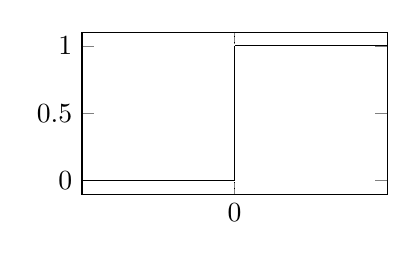
\begin{tikzpicture}
    	\begin{axis}[xmin=-5,xmax=5,xtick={0},xticklabels={0},height=0.3*\textwidth,width=0.45*\textwidth]
    		\addplot[domain=-5:0] {0};
            \addplot[domain=0:5] {1};
            \draw (axis cs:0,0) -- (axis cs:0,1);
            \draw[dotted] (axis cs:0,-1) -- (axis cs:0,2);
    	\end{axis}
    \end{tikzpicture}
    \label{fig:schwelle}
    }
    \subfigure[Sigmoid]{
    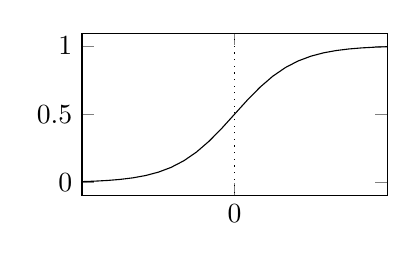
\begin{tikzpicture}
    	\begin{axis}[xmin=-5,xmax=5,xtick={0},xticklabels={0},height=0.3*\textwidth,width=0.45*\textwidth]
    		\addplot[] {1/(1+e^-x)};
            \draw[dotted] (axis cs:0,-1) -- (axis cs:0,2);
    	\end{axis}
    \end{tikzpicture}
    \label{fig:sigmoid}
    }\\\;\;
    \subfigure[ReLU]{
    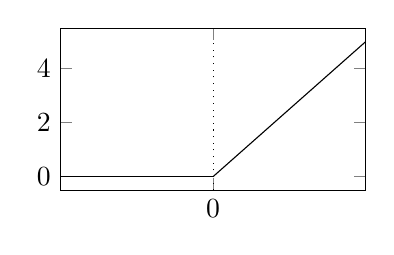
\begin{tikzpicture}
    	\begin{axis}[xmin=-5,xmax=5,xtick={0},xticklabels={0},height=0.3*\textwidth,width=0.45*\textwidth]
    		\addplot[domain=-5:0] {0};
            \addplot[domain=0:5] {x};
            \draw[dotted] (axis cs:0,-1) -- (axis cs:0,5);
    	\end{axis}
    \end{tikzpicture}
    \label{fig:relu}
    }
    \subfigure[Tanh]{
    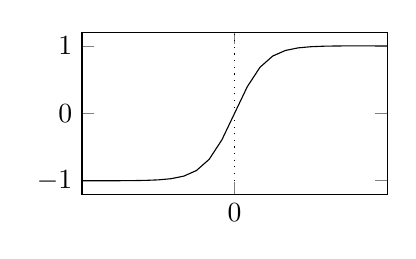
\begin{tikzpicture}
    	\begin{axis}[xmin=-5,xmax=5,xtick={0},xticklabels={0},height=0.3*\textwidth,width=0.45*\textwidth]
    		\addplot[domain=-5:5] {tanh(x)};
            \draw[dotted] (axis cs:0,-1) -- (axis cs:0,5);
    	\end{axis}
    \end{tikzpicture}
    \label{fig:tanh}
    }
    \caption{Graphen der Binären Stufen-, Sigmoid- und ReLU-Funktion}
    \label{fig:aktfunk}
\end{figure}
Die Sigmoidfunktion (siehe \ref{fig:sigmoid}) nimmt einen beliebigen Eingabewert und wandelt ihn in einen Ausgabewert zwischen 0 und 1 um. Sie ist besonders nützlich in der Ausgabeschicht von Klassifikationsproblemen, bei denen die Ausgabe eine Wahrscheinlichkeit ist.
Die Tanh-Funktion (dargestellt in \ref{fig:tanh}) wandelt, ähnlich wie die Sigmoid-Funktion, jeden Eingabewert in einen Ausgabewert zwischen -1 und 1 um, was sie nützlicher für Ausgaben macht, die sowohl positive als auch negative Werte annehmen sollen.
Im Gegensatz dazu gibt die ReLU-Funktion (vgl. \ref{fig:relu}) den Eingabewert unverändert zurück, wenn er positiv ist, und Null, wenn er negativ ist. Ein wesentlicher Vorteil der ReLU-Funktion ist, dass sie das Problem des verschwindenden Gradienten – bei dem die tiefen Schichten des Netzes nicht lernen – vermeidet, das bei älteren Aktivierungsfunktionen wie Tanh und Sigmoid auftritt \cite{atoum2023adaptive}. Außerdem hat sie einen geringeren Rechenaufwand.

Jede dieser Aktivierungsfunktionen hat ihre eigenen Eigenschaften und Verwendungszwecke, und die Wahl der richtigen Funktion hängt von dem spezifischen Problem und den Eigenschaften der Daten ab. In der Praxis werden häufig verschiedene Aktivierungsfunktionen in verschiedenen Schichten eines neuronalen Netzes verwendet, um die Leistung zu optimieren.
\section{Convolutional Neural Networks}
\label{sec:convnet}
CNNs sind eine Form künstlicher neuronaler Netze, die speziell für die Verarbeitung und Extraktion räumlicher Informationen aus Daten, insbesondere aus Bildern und anderen mehrdimensionalen Datenstrukturen, entwickelt wurden \cite{8308186}.
Sie sind ein wichtiger Bestandteil in vielen modernen maschinellen Lernsystemen, insbesondere im Bereich des maschinellen Sehens und haben wesentlich dazu beigetragen, die Leistungsfähigkeit von Algorithmen in Aufgaben wie Bild- und Videoklassifikation, Objekterkennung und Segmentierung zu verbessern \cite{oshea2015introduction}.

Das grundlegende Prinzip eines CNN besteht darin, kleine, lokalisierte Merkmale aus den Eingabedaten zu lernen und diese dann zu abstrahieren und zu kombinieren, um komplexere Muster und Strukturen zu erkennen. Ein CNN besteht typischerweise aus drei Arten von Schichten: Convolution-Schichten (Abbildung \ref{sec:conv}), Pooling-Schichten (dargestellt in \ref{sec:pool}) und Fully Connected-Schichten, die einem mehrschichtigen Perzeptron (Erklärung in \ref{sec:mehrperz}) ähnlich sind.

\subsection{Convolution-Schichten}
\label{sec:conv}
Convolution-Schichten sind entscheidend für die Extraktion von Merkmalen aus den Eingabedaten. Im Folgenden wird die Arbeitsweise näher erläutert.

In einer Faltungsschicht wird ein Filter – auch Kernel genannt –, der aus einer Matrix von Gewichten besteht, über die gesamte Eingabe geschoben. Dieser Vorgang wird als Convolution (Faltung) bezeichnet und ist in Abbildung \ref{fig:conv} dargestellt. Klassische Filtergrößen sind dabei 3×3, 5×5 oder 7×7. Die Filter sind daher in der Regel viel kleiner als die Eingabe, decken aber die gesamte Tiefe der Eingabe ab. Bei einem Farbbild beträgt die Tiefe beispielsweise drei.

Durch die Anwendung dieser Filter auf die Eingabedaten, identifizieren die\\Convolution-Schichten Muster, Kanten und Texturmerkmale. Die Simulation des Verschiebens der Filter über die Eingabedaten wird durch sogenannte rezeptive Felder simuliert. Dabei werden die Neuronen einer Schicht ausschließlich mit den Neuronen der vorhergehenden Schicht verbunden, die innerhalb des durch die Filtergröße definierten rezeptiven Feldes liegen. Diese lokale Verknüpfung ermöglicht es dem CNN, räumliche Informationen zu erfassen und lokal relevante Merkmale zu extrahieren, während gleichzeitig die Anzahl der zu lernenden Parameter durch die gemeinsame Nutzung von Parametern (da der Filter auf mehrere Bereiche des Bildes angewendet wird) reduziert wird \cite{weisstein_convolution}.

Um die Ausgabegröße der Convolution-Schichten zu steuern und sicherzustellen, dass sie genügend räumliche Information enthalten, können zwei wichtige Parameter verwendet werden: Padding und Stride.

\begin{figure}[htbp]
    \centering
    %\vspace{3cm}
    \begin{tikzpicture}[]%[scale = 0.7, transform canvas={scale=0.7}]
      % Padded input matrix
      \matrix (input) [matrix of nodes, nodes={draw, minimum size=.85cm}] {
        0 & 0 & 0 & 0 & 0 \\
        0 & 1 & 2 & 3 & 0 \\
        0 & 4 & 5 & 6 & 0 \\
        0 & 7 & 8 & 9 & 0 \\
        0 & 0 & 0 & 0 & 0 \\
      };
      % Kernel matrix
      \matrix (kernel) [right=2cm of input.north east, matrix of nodes, nodes={draw, minimum size=0.6cm}] {
        1 & 0 & -1\\
        2 & 0 & -2\\
        1 & 0 & -1\\
      };
      % Convolved matrix (with padding)
      \matrix (conv) [right=6cm of input, matrix of nodes, nodes={draw, minimum size=.88cm}] {
        -9 & -9 & 9 \\
        -20 & -8 & 20 \\
        -21 & -6 & 21 \\
      };
      % Labels
      \node[above=1ex of input, font=\large] {Padded Input};
      \node[above=1ex of kernel, font=\large] {Kernel};
      \node[above=1ex of conv, font=\large] {Output};
    
      % Convolution operation
      \begin{scope}[thick, red, on background layer]
        \node[draw, thick, fill=red!30, fit={(input-1-1) (input-3-3)}, inner sep=0pt] (box1) {};
        \node[draw, thick, red, fit={(kernel-1-1) (kernel-3-3)}, inner sep=0pt] (box2) {};
        \node[draw, thick, fill=red!30, fit={(conv-1-1) (conv-1-1)}, inner sep=0pt] (box3) {};
        \draw[thick, ->] (box1) -- (box2);
        \draw[thick, ->] (box2) -- (conv-1-1);
      \end{scope}
    \end{tikzpicture}
    %\hspace{5cm}
    %\vspace{2cm}
    \caption{Zero-padded Bild. Der Stride ist eins. Somit entspricht die Ausgangsgröße der Faltung der Eingangsgröße. Der Sobel-Operator wird als Kernel verwendet \cite{kanopoulos1988design}.}
    \label{fig:conv}
\end{figure}
Padding bezieht sich auf das Hinzufügen zusätzlicher Randpixel zur Eingabe, bevor der Filter angewendet wird. Dadurch wird sichergestellt, dass die Größe der Ausgabe erhalten bleibt, insbesondere wenn der Filter über die Ränder der Eingabe gleitet \cite{convolution}.

Stride bezieht sich auf die Anzahl der Pixel, um die der Filter bei jedem Schritt über die Eingabe gleitet. Ein Stride von eins bedeutet, dass der Filter Pixelweise verschoben wird, während ein größerer Stride zu größeren Schritten führt. Ein größerer Stride reduziert die räumliche Dimension der Ausgabe, da weniger Positionen des Filters überprüft werden. Dadurch kann die Größe der Netzarchitektur reduziert werden \cite{convolution}.

\subsubsection{Dilated-Convolution}
\label{sec:dilconv}
Dilated Convolution, auch bekannt als Atrous Convolution, ist eine von Yu \textit{et al.} entwickelte Technik zur effektiven Erweiterung des Rezeptiven Feldes in einer CNN-Architektur, ohne dabei die räumliche Auflösung zu verlieren oder die Anzahl der Parameter zu erhöhen \cite{yu2015multi}.
\begin{figure}[htbp]
    \centering
    \includegraphics[width=.7\linewidth]{img/dilconv.png}
    \captionsource{(a) 1-dilated convolution mit 3x3 rezeptivem Feld, (b) 2-dilated convolution mit 7x7 rezeptivem Feld, (c) 4-dilated convolution mit 15x15 rezeptivem Feld}{Dilated Residual Networks \cite{Yu_2017_CVPR}}
    \label{fig:dilconv}
\end{figure}
Die Technik verwendet eine sogenannte Verdünnungsrate (dilation rate), die die Abstände zwischen den Gewichten in der Filtermaske vergrößert. Ein Beispiel ist in Abbildung \ref{fig:dilconv} dargestellt. Durch die Anwendung von Dilated-Convolutions kann das Netz somit mehr Kontextinformation aus dem Eingabebild extrahieren, ohne die Komplexität des Netzes wesentlich zu erhöhen. Yu \textit{et al.} zeigen, dass diese Technik besonders wertvoll in Anwendungen ist, die eine detaillierte Segmentierung erfordern, da sie es ermöglicht, Informationen über größere Eingangsbereiche zu sammeln und gleichzeitig eine hohe Auflösung in der Ausgabe beizubehalten \cite{Yu_2017_CVPR}. Insbesondere bei Aufgaben, bei denen es auf die genaue Lokalisierung von Objekten ankommt, wie beispielsweise der Spitzenerkennung in Nanoprobing-Anwendungen, kann der Einsatz von Dilated-Convolutions zu verbesserten Ergebnissen führen.

\subsection{Pooling-Schichten}
\label{sec:pool}
Pooling-Schichten bilden einen weiteren wichtigen Bestandteil von CNNs, sie werden dazu genutzt, die Dimension der von Convolution-Schichten erzeugten Featuremaps zu reduzieren und gleichzeitig wichtige Merkmale beizubehalten \cite{pooling}. Dies wird erreicht, indem benachbarte Werte über eine Funktion reduziert werden. Die häufigsten Pooling-Operationen sind das Max-Pooling und das Average-Pooling.\\
\begin{figure}[htbp]
    \centering
    \vspace{0cm}
    \begin{tikzpicture}[]%[scale = 0.7, transform canvas={scale=0.7}]
      % Input matrix
      \matrix (input) [matrix of nodes, nodes={draw, minimum size=.8cm}] {
        7 & 3 & 9 & 1 \\
        4 & 6 & 2 & 8 \\
        2 & 5 & 7 & 3 \\
        8 & 1 & 5 & 9 \\
      };
      % Max-Pooled matrix
      \matrix (maxpooled) [above right=2cm of input.east, matrix of nodes, nodes={draw, minimum size=.8cm}] {
        7 & 9 \\
        8 & 9 \\
      };
    
      % Pooled matrix
      \matrix (avgpooled) [below right=2cm of input.east, matrix of nodes, nodes={draw, minimum size=.8cm}] {
        5 & 5 \\
        4 & 6 \\
      };
      
      % Labels
      \node[above=1ex of input, font=\large] {Input};
      \node[above=1ex of maxpooled, font=\large] {Max Pooled};
      \node[above=1ex of avgpooled, font=\large] {Average Pooled};
    
      % Pooling operation
      \begin{scope}[thick, red, on background layer]
        \node[draw, thick, fill=red!30, fit={(input-1-1) (input-2-2)}, inner sep=0pt] (box1) {};
        \node[draw, thick, fill=red!30, fit={(maxpooled-1-1)}, inner sep=0pt] (box2) {};
        \node[draw, thick, fill=red!30, fit={(avgpooled-1-1)}, inner sep=0pt] (box8) {};
        
        \node[draw, thick, fill=yellow!30, fit={(input-1-3) (input-2-4)}, inner sep=0pt] (box3) {};
        \node[draw, thick, fill=yellow!30, fit={(maxpooled-1-2)}, inner sep=0pt] (box4) {};
        \node[draw, thick, fill=yellow!30, fit={(avgpooled-1-2)}, inner sep=0pt] (box9) {};
        
        \node[draw, thick, fill=blue!30, fit={(input-3-1) (input-4-2)}, inner sep=0pt] (box4) {};
        \node[draw, thick, fill=blue!30, fit={(maxpooled-2-1)}, inner sep=0pt] (box5) {};
        \node[draw, thick, fill=blue!30, fit={(avgpooled-2-1)}, inner sep=0pt] (box10) {};
        
        \node[draw, thick, fill=green!30, fit={(input-3-3) (input-4-4)}, inner sep=0pt] (box6) {};
        \node[draw, thick, fill=green!30, fit={(maxpooled-2-2)}, inner sep=0pt] (box7) {};
        \node[draw, thick, fill=green!30, fit={(avgpooled-2-2)}, inner sep=0pt] (box11) {};
      \end{scope}
      \draw[thick, ->] (box1) -- (box2);
      \draw[thick, ->] (box1) -- (box8);
    \end{tikzpicture}
    \hspace{0cm}
    \vspace{0cm}
    \caption{Pooling dient der Dimensionsreduktion unter Beibehaltung der aussagekräftigsten Merkmale, wobei Methoden wie Max-Pooling und Average-Pooling zum Einsatz kommen.}
    \label{fig:pad}
\end{figure}
Beim Max-Pooling wird in jedem Pooling-Bereich der maximale Wert als repräsentativer Wert verwendet. Dies hilft dabei, herausragende Merkmale oder Aktivierungen hervorzuheben und die Positionsinformationen zu erhalten.
Beim Average-Pooling wird hingegen der Durchschnitt der Werte im Pooling-Bereich berechnet. Dadurch werden die Werte geglättet und das Netzwerk wird robuster gegenüber kleinen lokalen Verschiebungen.
Über die Kernelgröße, den Stride und das Padding kann die Ausgabegröße der Pooling-Schicht wie bei der Convolution bestimmt werden.
\clearpage
\section{Mask R-CNN}
Mask R-CNN ist ein innovativer Ansatz für Instanzsegmentierungsaufgaben, der auf dem Konzept der Region Based Convolutional Neural Networks (R-CNNs) basiert \cite{Girshick_2015_ICCV}\cite{7112511}. Mask R-CNN wurde 2017 von He \textit{et al.} bei Facebook AI Research entwickelt und erstmals veröffentlicht \cite{He_2017_ICCV}. Es stellt einen Meilenstein in der Entwicklung von Algorithmen zur Objekterkennung und -segmentierung dar.
Mask R-CNN erweitert und verbessert das von Ren \textit{et al.} entwickelte Modell Faster R-CNN \cite{DBLP:journals/corr/RenHG015} in mehreren Punkten.
\begin{figure}[htbp]
    \centering
    \includegraphics[width=\linewidth]{img/maskrcnn_network_custom.png}
    \captionsource{Mask R-CNN Architektur}{Modifiziert aus der MathWorks Dokumentation \cite{mathworks-maskrcnn}}
    \label{fig:maskrcnn}
\end{figure}
Dem Modell wird ein zusätzlicher Segmentierungszweig hinzugefügt, der es ermöglicht, für jedes erkannte Objekt eine präzise, pixelgenaue Maske zu erzeugen. Diese Eigenschaft unterscheidet Mask R-CNN von Faster R-CNN und erweitert dessen Fähigkeiten über die reine Objekterkennung und -klassifikation hinaus. Darüber hinaus implementiert Mask R-CNN eine sogenannte RoIAlign Schicht, um das Problem der Diskrepanz zwischen dem RoIPooling in Faster R-CNN und der pixelgenauen Segmentierung zu lösen, was zu einer weiteren Verbesserung der Modellleistung führt. Die Implementierung von RoIAlign wird im Rahmen dieser Arbeit nicht weiter behandelt und kann in dem von He \textit{et al.} veröffentlichten Paper \cite{He_2017_ICCV} entnommen werden.
\subsection{Backbone Netzwerk}
\label{sec:backbone}
Das Backbone-Netz wird verwendet, um tief abstrahierte Merkmale aus den Eingabedaten zu extrahieren. Es stellt die erste Stufe von Mask R-CNN dar. In Abbildung \ref{fig:maskrcnn} ist sie als \glqq CNN\grqq{} linken dargestellt.
Die extrahierten Merkmale dienen als Input für den Rest des Netzes, das spezifische Aufgaben wie Objekterkennung, Segmentierung oder Klassifikation durchführt.
Die Wahl des Backbone-Netzes hat einen wesentlichen Einfluss auf die Leistungsfähigkeit des Gesamtsystems. Sie hängt von der Komplexität des Problems, den spezifischen Anforderungen der Aufgabe und der Rechenkapazität ab.

Residuale Netzwerke (ResNet) welche erstmal von He \textit{et al.} vorgestellt wurden \cite{He_2016_CVPR}, lösen das Problem des vanishing/exploding Gradienten \cite{7112511} in tiefen Netzen durch die Nutzung von skip-connections \cite{1603.05027}\cite{1701.09175}\cite{1507.06228}. Sie sind eine weit verbreitete Wahl für die Objektdetektion und -segmentierung \cite{2206.08016}.
ResNets gibt es in verschiedenen Tiefen, darunter Modelle wie ResNet-50 und ResNet-101, wobei sich jede Zahl auf die Anzahl der Convolution-Schichten im Netzwerk bezieht. Tiefere Modelle können in der Regel komplexere Merkmale erfassen, benötigen jedoch mehr Rechenleistung und Speicherplatz.

\begin{figure}[htbp]
    \centering
    \includegraphics[width=\linewidth, angle=180]{img/resnet34.png}
    \captionsource{Architektur des ResNet-34. ResNet Netze bestehen aus mehreren Ebenen. Jede Ebene extrahiert Merkmale auf einer anderen Abstraktionsebene.}{\cite{He_2016_CVPR}}
    \label{fig:resnet34}
\end{figure}
ResNet-FPN, wobei FPN für Feature Pyramid Network steht, ist eine Variante des ResNet-Modells, die speziell für Aufgaben entwickelt wurde, die eine Objekterkennung auf unterschiedlichen Skalen erfordern. Ein FPN verbessert die Fähigkeit von ResNets, Objekte unterschiedlicher Größe zu erkennen, indem eine Pyramide von Feature-Maps erzeugt wird, die von der hochauflösenden, semantisch schwachen Ebene bis zur niedrigauflösenden, semantisch starken Ebene reicht. Für weitere Informationen zu FPN siehe \cite{1612.03144}.

Eine weitere für diese Arbeit relevante Variante der ResNet-Architektur ist ResNet-DC5. Diese Konfiguration enthält – anstelle von FPN – Dilated Convolutions \ref{sec:dilconv} in der C5-Ebene von ResNet. Die Integration von Dilated Convolutions ermöglicht es dem Netzwerk, mehr Kontextinformationen aus dem Eingabebild zu extrahieren und somit feinere Details in den Daten zu erkennen. Dies ist besonders vorteilhaft für Aufgaben, bei denen präzise Informationen benötigt werden.
\subsection{Region Proposal Netzwerk}
Das Region Proposal Network (RPN) ist ein Schlüsselelement in der Architektur von Mask R-CNN. Es ist dafür verantwortlich, Regionen von Interesse (RoI) innerhalb des Bildes zu identifizieren, die potenziell Objekte enthalten könnten. Dieses Netzwerk nimmt die extrahierten Merkmale des Backbone-Netzwerks als Eingabe und gibt eine Reihe von Rechtecken (Bounding Boxes) und Objektivitätsscores aus, die die Wahrscheinlichkeit angeben, mit der ein Objekt in dem jeweiligen Rechteck enthalten ist \cite{Hosang_2016}.
Die vorgeschlagenen Regionen werden durch die RoIAlign Technik mit den Merkmalen, die durch das Backbone extrahiert wurden, verbunden und werden für die anschließende Objektklassifikation und Segmentierung durch die nachfolgenden Stufen des Mask R-CNN Modells verwendet.

\subsection{Vortraining}
Die Verwendung vortrainierter Modelle ist eine gängige Praxis im maschinellen Lernen und insbesondere im Deep Learning, da sie erhebliche Vorteile bietet. Der Hauptvorteil ist die erhebliche Zeit- und Rechenersparnis, da das Netz nicht von Grund auf neu trainiert werden muss. Vortrainierte Modelle haben bereits eine Vielzahl von Merkmalen gelernt, die in verschiedenen Kontexten und für eine Vielzahl von Aufgaben nützlich sein können, und führen daher oft zu besseren Ergebnissen.
Darüber hinaus hilft die Verwendung von vortrainierten Modellen, das Problem der Überanpassung zu reduzieren, insbesondere wenn die Menge der verfügbaren Trainingsdaten begrenzt ist.

Für das Mask R-CNN Vortraining wird häufig der COCO-Datensatz \cite{coco} verwendet, der eine Vielzahl von Objektkategorien aus unterschiedlichen Kontexten enthält. Dies bietet eine gute Grundlage für die Erkennung und Segmentierung verschiedener Objekttypen in den meisten gängigen Szenarien. Ein weiteres beliebtes Vortraining ist das auf dem ImageNet-Datensatz \cite{deng2009imagenet}, der Millionen von Bildern aus Tausenden von Kategorien enthält. Diese vortrainierten Modelle können dann für die spezifischen Anforderungen einer bestimmten Aufgabe weiter trainiert werden, ein Prozess, der auch als Fine-Tuning bezeichnet wird.
\subsection{Hyperparameter}
Die Wahl der richtigen Hyperparameter ist entscheidend für das Training von Deep Learning Modellen und kann einen großen Einfluss auf die Leistung des Modells haben.

Ein essenzieller Parameter beim Training von neuronalen Netzen ist die Lernrate. Die Lernrate gibt an, wie stark die Gewichte des Modells in jedem Trainingsschritt angepasst werden. Ein zu hoher Wert kann dazu führen, dass das Modell die optimale Lösung \glqq überspringt\grqq{}, während ein zu niedriger Wert zu einem sehr langsamen Lernfortschritt führen kann \cite{learnrate}.

Momentum ist eine gängige Technik zur Überwindung lokaler Minima im Optimierungsprozess und beschleunigt die Konvergenz des Modells \cite{pmlr-v119-cutkosky20b}\cite{pmlr-v28-sutskever13}.
Ein weiterer Parameter für das effizientere Training ist die Gewichtsabnahme. Sie ist eine Form der Regularisierung, die dazu beiträgt, die Komplexität des Modells zu kontrollieren und Overfitting zu vermeiden, indem kleine Strafen auf die Modellgewichte angewendet werden \cite{Ying_2019}\cite{doi:10.1021/ci0342472}.

Die Batch-Größe bestimmt die Anzahl der Bilder, die das Modell verarbeitet, bevor seine Gewichte aktualisiert werden. Sie hat einen großen Einfluss auf die Konvergenz und Genauigkeit des Modells \cite{KANDEL2020312}.
\subsection{Trainingsablauf}
% Der Trainingsprozess des Mask R-CNN Modells verwendet eine Reihe von Verlustfunktionen, um das Modell für die genaue Erkennung und Segmentierung von Objekten zu trainieren. Zu diesen Verlustfunktionen gehören der\\RPN-Klassifikationsverlust, der RPN-Regressionsverlust, der Klassifikationsverlust, der Box-Regressionsverlust und der Maskenverlust \cite{Girshick_2015_ICCV} \cite{Wang.2022}. Jede dieser Funktionen wurde entwickelt, um einen bestimmten Aspekt des Modells zu optimieren.

% Für das Training des Modells wird in der Regel das Verfahren Stochastic Gradient Descent (SGD) oder eine seiner Varianten wie Adam \cite{AMARI1993185} \cite{kingma2017adam} verwendet. Das Modell wird dabei auf einen Trainingsdatensatz angewendet, und die Verlustfunktionen bewerten, wie gut die Vorhersagen des Modells mit den tatsächlichen Werten übereinstimmen. Die Gewichte und Bias-Werte des Modells werden mittels Backpropagation \cite{Rumelhart.1986} entsprechend angepasst, um die Verluste zu minimieren und damit die Leistung zu verbessern.

% Es ist üblich, das Training fortzusetzen, bis auf einem Validierungsdatensatz keine erkennbare Verbesserung mehr erzielt wird. Dies deutet darauf hin, dass das Modell einen Punkt erreicht hat, an dem es beginnt, sich an die Trainingsdaten über anzupassen.

% Um eine optimale Konvergenz zu erreichen, kann die Lernrate, die die Schrittgröße bei der Optimierung bestimmt, während des Trainings angepasst werden. Häufig wird die Lernrate schrittweise verringert, um die Bewegungen in Richtung des optimalen Minimums der Verlustfunktion zu verfeinern. Dieser Prozess hilft, das Modell in Richtung einer besseren Leistung und Generalisierungsfähigkeit zu lenken.

% Insgesamt durchläuft das Modell während des Trainingsprozesses einen iterativen Zyklus der Parameteranpassung, um die Verlustfunktionen zu minimieren. Dies führt zu einer schrittweisen Verbesserung der Modellleistung bei der Erkennung und Segmentierung von Objekten mit komplexen Eigenschaften.
Der Trainingsprozess des Mask R-CNN Modells verwendet Verlustfunktionen, um die Erkennung und Segmentierung von Objekten zu optimieren. Dazu gehören der RPN-Klassifikations- und RPN-Regressionsverlust, der Klassifikationsverlust, der Box-Regressionsverlust und der Maskenverlust \cite{Girshick_2015_ICCV} \cite{Wang.2022}. Üblicherweise werden Stochastic Gradient Descent (SGD) oder Varianten wie Adam zum Training verwendet \cite{AMARI1993185} \cite{kingma2017adam}. Dabei wird das Modell auf einem Trainingsdatensatz trainiert, die Gewichte und Bias-Werte werden durch Backpropagation angepasst, um Verluste zu minimieren \cite{Rumelhart.1986}.

Das Training wird fortgesetzt, bis auf einem Validierungsdatensatz keine Verbesserung mehr erzielt wird. Die Lernrate des Modells kann angepasst werden und wird häufig schrittweise verringert, um die Optimierung zu verfeinern. Insgesamt besteht der Prozess aus einem iterativen Zyklus der Parameteranpassung, um eine kontinuierliche Verbesserung der Modellleistung bei der Erkennung und Segmentierung komplexer Objekte zu erreichen.
\section{Datensatz}
Für viele Aufgaben des maschinellen Sehens sind bereits große Datensätze frei verfügbar, die Tausende von Bildern mit Objekten enthalten und zum Training eigener Netze verwendet werden können \cite{paperswithcode-datasets} \cite{bioimage-datasets}. Im Bereich des Nanoprobings ist derzeit jedoch kein geeigneter Datensatz verfügbar. Die Erstellung eines Datensatzes ist daher Teil dieser Arbeit. Dazu wurde das im folgenden Abschnitt beschriebene Format verwendet.
\subsection{COCO Data Annotation Format}
Das Common Objects in Context (COCO) Data Annotation Format ist ein weit verbreitetes Format für die Annotation von Bilddaten, das häufig für maschinelles Sehen und Deep Learning verwendet wird. COCO bietet eine umfangreiche Sammlung von Annotationen, einschließlich Objekterkennung, Segmentierung und Schlüsselpunkterkennung \cite{coco}.
Das im Rahmen dieser Arbeit verwendete Format, welches in Abbildung \ref{fig:datform} zu sehen ist, ist abgeleitet von COCO und angepasst an die spezifischen Anforderungen.

Bei der Bounding-Box-Annotation werden die Koordinaten als x- und y-Position des oberen linken Punktes sowie als Breite und Höhe der Box angegeben. Für die Segmentierung wird eine Liste von Punktkoordinaten verwendet, die den Umriss des Objekts definieren. Ein Keypoint wird durch ein Tupel von drei Werten (x, y, v) dargestellt. Dabei sind x und y die Koordinaten des Keypoints im Bild.\\Der Wert v ist ein Sichtbarkeitsflag, das den Status des Keypoints angibt. Er kann drei verschiedene Werte annehmen: 0, wenn der Keypoint im Bild nicht vorhanden ist; 1, wenn der Keypoint vorhanden, aber nicht sichtbar ist; und 2, wenn der Keypoint vorhanden und sichtbar ist.



\subsection{Evaluationsmetriken}
Die Bewertung von Objekterkennungs-, Segmentierung- und Schlüsselpunktvorhersagemodellen erfordert präzise Metriken, um ihre Leistung objektiv zu bewerten. Im Rahmen des COCO-Datenformats werden verschiedene Evaluationsmetriken verwendet, um die Qualität der Ergebnisse zu quantifizieren \cite{coco}.
\subsubsection{Intersection over Union}

% \begin{figure}[htbp]
%     \centering
%     \includegraphics[width=.2\linewidth]{img/IoU.png}
%     \caption{Visualisierung der Intersection over Union}
%     \label{fig:jaccard}
% \end{figure}
Die Metrik Intersection over Union (IoU) – auch Jaccard-Koeffizient genannt – bewertet die räumliche Übereinstimmung zwischen den vorhergesagten (A) und den tatsächlichen (B) Bounding Boxen oder Masken der Objekte.
\begin{equation}
    \text{IoU}(A, B) = \dfrac{{A \cap B}}{{A \cup B}}
\end{equation}
Der IoU wird berechnet, indem die Fläche der Überlappung durch die Fläche der Vereinigung dividiert wird. Ein hoher IoU-Wert zeigt eine hohe Übereinstimmung zwischen den vorhergesagten und den tatsächlichen Bereichen an. Im Zusammenhang mit der Objekterkennung und Segmentierung wird der IoU verwendet, um zu bestimmen, ob eine vorhergesagte Bounding Box oder Maske als korrekt angesehen wird.

\subsubsection{Object Keypoint Similarity}

Die Metrik Object Keypoint Similarity (OKS) bewertet die Vorhersage von Schlüsselpunkten anhand einer normalisierten Distanz zwischen den vorhergesagten und den tatsächlichen Schlüsselpunkten eines Objekts. Sie spielt damit die gleiche Rolle wie die IoU. Die OKS wird mit folgender Formel berechnet:

\begin{equation}
    \text{OKS} = \frac{{\sum_{i}{\exp\left(-\frac{{d_i^2}}{{2s^2\kappa_i^2}}\right)\delta(v_i > 0)}}}{{\sum_{i}{\delta(v_i > 0)}}}
\end{equation}


Dabei ist \(d_i \) der Abstand zwischen den Schlüsselpunkten, \(s \) der Objektmaßstab, \(\kappa_i \) eine Normierungskonstante und \(\delta \) die Indikatorfunktion für sichtbare Schlüsselpunkte (\(v_i\) ist der Sichtbarkeitsflag). Die Normierungskonstante bestimmt, wie empfindlich die OKS auf Abweichungen des vorhergesagten Punktes von dem wahren Punkt reagiert.
Ein hoher OKS-Wert zeigt an, dass die vorhergesagten Schlüsselpunkte gut mit den tatsächlichen Schlüsselpunkten übereinstimmen, wobei sowohl die Genauigkeit als auch die Standardabweichung berücksichtigt werden.
Für eine ausführliche Erklärung der OKS wird auf die offizielle COCO Dokumentation verwiesen \cite{coco}.
% \begin{figure}[htbp]
%     \centering
%     \includegraphics[width=0.3\linewidth, trim={5cm 4cm 10cm 0},clip, angle=90]{img/oks1.png}
%     \captionsource{Exemplarische Darstellung der OKS. Die roten Kreise stellen verschiedene Standardabweichungen dar, die durch \(\sigma\) festgelegt werden.}{Kleindiek Nanotechnik GmbH}
%     \label{fig:oks}
% \end{figure}
\subsubsection{Average Precision}
Die Metrik Average Precision (AP) ist eine zentrale Evaluationsmetrik für die Bewertung von Objekterkennungsmodellen. Sie misst die Genauigkeit der Objektlokalisierung und -klassifizierung unter Berücksichtigung von False Positives (FP) und False Negatives (FN). Die AP wird aus der Fläche unter der Precision-Recall-Kurve berechnet, wobei Precision und Recall durch die folgenden Formeln definiert sind:

\begin{multicols}{2}
\begin{equation}    
\begin{aligned}
    \text{Precision}&=\dfrac{\text{TP}}{\text{TP}+\text{FP}}\\
        &=\dfrac{\text{TP}}{\text{\#Vorhersagen}}
\end{aligned}
\label{eq:precision}
\end{equation}\break
\begin{equation}    
\begin{aligned}
    \text{Recall}&=\dfrac{\text{TP}}{\text{TP}+\text{FN}}\\
        &=\dfrac{\text{TP}}{\text{\#Ground Truth}}
\end{aligned}
\label{eq:recall}
\end{equation}
\end{multicols}

Die Precision (\ref{eq:precision}) gibt an, wie viele der vorhergesagten Objekte tatsächlich korrekt sind, während der Recall (\ref{eq:recall}) angibt, wie viele der tatsächlich vorhandenen Objekte korrekt vorhergesagt wurden.
Berechnet man diese zwei Werte für die akkumulierten Vorhersagen des Modells und zeichnet sie in einem Diagramm auf, erhält man die Precision-Recall-Kurve.

AP wird sowohl bei der Objekterkennung als auch bei der Schlüsselpunktvorhersage verwendet, um die Gesamtleistung der Modelle zu bewerten. Es gibt sie in verschiedenen Varianten. Die für diese Arbeit relevanten AP-Metriken sind in Tabelle \ref{tab:AP} aufgelistet.
\begin{table}[h]
    \centering
    \begin{tabular}{ll}
        \toprule
        \textbf{Metrik}                 & \textbf{Beschreibung}                               \\
        \midrule
        $\text{AP}$                & AP at IoU=.50:.05:.95 (primary challenge metric)      \\
        $\text{AP}^{IoU=.50}$                & AP at IoU=.50 (PASCAL VOC metric)                     \\
        $\text{AP}^{IoU=.75}$                & AP at IoU=.75 (strict metric)                         \\
        $\text{AP}$                       & AP at OKS=.50:.05:.95 (primary challenge metric)      \\
        $\text{AP}^{OKS=.50}$                & AP at OKS=.50 (loose metric)                          \\
        $\text{AP}^{OKS=.75}$                & AP at OKS=.75 (strict metric)                         \\
        \bottomrule
    \end{tabular}
    \captionsource{Übersicht der für diese Arbeit relevanten Average Precision (AP) Metriken}{COCO Dokumentation \cite{coco}}
    \label{tab:AP}
\end{table}

\begin{figure}[h]
    \centering
    \begin{minipage}{0.43\textwidth}
        \begin{lstlisting}[language=json,firstnumber=1]
{
  "images": [
    {
      "id": int,
      "width": int,
      "height": int,
      "file_name": str
    }
  ],
  "categories": [
    {
      "id": int,
      "name": str,
      "supercategory": str,
      "keypoints": [str],
      "skeleton": [edge]
    }
  ],
        \end{lstlisting}
    \end{minipage}\hfill
    \begin{minipage}{0.53\textwidth}
        \begin{lstlisting}[language=json,firstnumber=19]
  "annotations": [
    {
      "id": int,
      "image_id": int,
      "category_id": int,
      "segmentation": [polygon],
      "area": float,
      "bbox": [x, y, width, height],
      "iscrowd": 0 or 1,
      "keypoints": [x1,y1,v1,..],
      "num_keypoints": int,
    }
  ]
}
    \end{lstlisting}
    \vspace{1.6cm}
    \end{minipage}
    \caption{Das in dieser Arbeit verwendete Annotation Format, abgespeichert als JSON Datei. Datensätze in COCO Format können mit den meisten Frameworks nativ zum Training Neuronaler Netze verwendet werden.}
    \label{fig:datform}
\end{figure}
\clearpage
\chapter{Verwandte Werke}

\section{Detektion und Segmentierung von Mitochondrien in Rasterelektronenmikroskop Bildern}
In der Arbeit \glqq Automatic Detection and Segmentation of Mitochondria from SEM Images using Deep Neural Network\grqq{} widmen sich Liu \textit{et al.} der Herausforderung, Mitochondrien in hochauflösenden REM-Bildern automatisch zu erkennen und zu segmentieren \cite{8512393}. Sie stellen fest, dass trotz erheblicher Fortschritte die Komplexität der Zellstrukturen, das Hintergrundrauschen und Bildartefakte diese Aufgabe nach wie vor erschweren.
Um dieses Problem zu lösen, schlagen die Autoren einen verbesserten Mask R-CNN Ansatz vor. Dieses Modell ist eine Weiterentwicklung der von He \textit{et al.} \cite{He_2017_ICCV} vorgestellten Mask R-CNN Architektur und beinhaltet neben der Erkennung und Segmentierung von Mitochondrien auch eine morphologische Verarbeitung und die Einbeziehung von Kontextinformationen zur Korrektur lokaler Fehleinschätzungen. Ein besonderes Merkmal dieses Ansatzes ist die Nutzung des Field of View (FoV) der Maskenverzweigung zur Erzeugung mehrerer Maskenausgaben in vier Richtungen, die für die abschließende Segmentierung kombiniert werden.

Die Validierungsergebnisse, basierend auf zwei gängigen Datensätzen, zeigen, dass der vorgeschlagene Ansatz eine vergleichbare Leistung wie die bisher besten Methoden erreicht. Darüber hinaus konnten Mitochondrien verschiedener Größen und Maßstäbe erfolgreich detektiert und segmentiert werden, wobei geeignete Nachbearbeitungsverfahren eine deutliche Verbesserung der Segmentierungsleistung ermöglichten.
Die vorgestellte Methode in der Arbeit unterstreicht die Effektivität von Deep Learning-Modellen, wie Mask R-CNN, bei der Bewältigung der Herausforderungen der Segmentierung in hochauflösenden REM-Bildern. Durch die gezielte Anpassung und Optimierung dieses Modells für die spezifischen Aufgaben der Mitochondrien-Erkennung konnten die Autoren bemerkenswerte Ergebnisse erzielen.
Diese Ergebnisse lassen darauf schließen, dass ähnliche Anpassungen des Modells es ebenso ermöglichen könnten, die Lokalisierung und Identifizierung von Messpitzen in REM-Bildern zu automatisieren und zu verbessern. Daher könnte die hier dargelegte Vorgehensweise einen vielversprechenden Ausgangspunkt für die Anpassung von Deep Learning-Modellen an die spezifischen Anforderungen der Messpitzen-Lokalisierung bieten.

\newpage
%\section{ZeroCostDL4Mic}
\section{FibeR-CNN}
Mit der Arbeit \glqq FibeR-CNN: Expanding Mask R-CNN to Improve Image-Based Fiber Analysis\grqq{} leisten Frei und Kruis einen wichtigen Beitrag zur Herausforderung der automatisierten Bildanalyse von faserförmigen Materialien in REM-Bildern. Sie identifizieren einen Mangel an effektiven automatisierten Algorithmen zur Bildannotation von überlappenden und verdeckten Fasern, die eine genaue Bestimmung der Faserlänge und -breite ermöglichen \cite{Frei_2021}. Bestehende Methoden wie CTFIRE sind nicht nur unzureichend, sondern auch sehr zeitaufwendig.
Um dieses Problem zu lösen, erweitern die Autoren die Mask R-CNN Architektur innerhalb des Detectron2 Frameworks und entwickeln einen spezifischen Ansatz für die Analyse von Faserbildern, den sie FibeR-CNN nennen \cite{wu2019detectron2}\cite{fiberrcnn}.

FibeR-CNN wurde so modifiziert, dass es zusätzlich zur Segmentierung auch die Breite und Länge der Fasern vorhersagen kann. Durch die Verwendung von CNNs erweist sich der Ansatz als robust gegenüber Änderungen der Bildbedingungen und benötigt nach dem Training keine Parameteranpassung durch den Benutzer. Somit ist es ein effektives Werkzeug für die automatische, bildbasierte Faserformanalyse.
Obwohl FibeR-CNN nicht direkt als Grundlage für diese Arbeit dient, bietet es wertvolle Einblicke, wie Mask R-CNN für spezifische Anforderungen in der REM-Bildsegmentierung modifiziert werden kann. Darüber hinaus bestätigt es, dass Mask R-CNN effektiv zur Segmentierung komplexer Strukturen in REM-Bildern eingesetzt werden kann, was Parallelen zur Aufgabe der Spitzenerkennung aufweist.
\section{Detectron2}
Detectron2 ist ein Open-Source-Software-Framework, das von der Facebook AI Research Group entwickelt wurde. Es bietet eine flexible, modulare und erweiterbare Architektur, die eine einfache Anpassung und Erweiterung verschiedener Modelle ermöglicht und die Entwicklung und das Experimentieren mit neuen Modellen und Algorithmen erleichtert. Detectron2 enthält Implementierungen der neuesten Objekterkennungs- und Segmentierungsalgorithmen, einschließlich Mask R-CNN und Faster R-CNN, und hat den Vorteil, dass es eine Reihe von vortrainierten Modellen bietet, die auf großen und unterschiedlichen Datensätzen wie COCO trainiert wurden. Durch die Verwendung von Detectron2 kann das Modell von diesen vortrainierten Gewichten profitieren, was den Trainingsprozess beschleunigt und die Modellleistung verbessert. Die in Detectron2 integrierten Werkzeuge für Training, Inferenz und Evaluierung sowie die umfangreichen Datenverarbeitungsfunktionen machen Detectron2 zu einem umfassenden Werkzeug, das den gesamten Prozess der Modellerstellung und -evaluierung erleichtert. Detectron2 bietet eine nahtlose Integration und Interoperabilität mit dem PyTorch Ökosystem \cite{wu2019detectron2}.
\clearpage
\chapter{Durchführung}
Die Erstellung eines Datensatzes für das Nanoprobing stellt eine Herausforderung dar, da eine große Anzahl von Bildern aus verschiedener Szenen erforderlich ist. Die manuelle Bewegung der Manipulatoren sowie die Steuerung des REM ist zeitaufwändig und erfordert viel Geschick, was die Erstellung eines umfangreichen Datensatzes erschwert.
Daher wurde eine Lösung benötigt, um die Bewegung der Manipulatoren und die Steuerung des REM zu automatisieren.
Verschiedene Ansätze wurden in Betracht gezogen, einschließlich der Verwendung der offiziell bereitgestellten Programme. Letztendlich wurde jedoch die Implementierung der Schnittstellen in Python als beste Lösung identifiziert.
Diese Schnittstellen ermöglichen die Fernsteuerung der Manipulatoren und des REM mittels eigens entwickelter Skripte, was die Erstellung eines umfangreichen Datensatzes erheblich erleichtert.
Um diese Daten effizient zu nutzen, werden verschiedene vortrainierte Varianten des Mask R-CNN Modells mit dem Detectron2 Framework trainiert und evaluiert.

In den folgenden Abschnitten dieses Kapitels wird die Umsetzung der verschiedenen Komponenten dieser Arbeit, einschließlich der Datenerfassung und des Modelltrainingsverfahrens, detailliert beschrieben.

%\newpage
\section{Implementierung der Nanocontrol Schnittstelle in Python}
Da es sich beim Nanocontrol um ein COM-Gerät handelt, wird zur Steuerung des Manipulators, auf dem die Messspitzen montiert sind, eine spezielle Schnittstelle in Python implementiert. Hierzu wird das Paket pySerial verwendet.

Die Kommunikation mit dem Nanocontrol über die COM-Schnittstelle basiert auf einem speziellen Befehls- und Antwortformat.
Die Befehle, die an das Nanocontrol gesendet werden, folgen dem Format \textbf{<command string><blank><param><CR>}, während die Antworten der das Format \textbf{<status char><tab><message string><CR>} haben.
Die Befehle decken eine Vielzahl von Funktionen ab, von der Abfrage von Informationen wie dem Systemstatus oder der Position des Manipulators bis hin zu spezifischen Befehlen für die Bewegung des Manipulators.

\begin{figure}[h]
    \centering
    \includegraphics[width=\linewidth]{img/nc_func.png}
    \captionsource{Befehle, um die Position der Manipulatoren im Grob- und Feinbereich auszulesen und zu ändern. Auszug dem Nanocontrol Software Manual.}{Kleindiek Nanotechnik GmbH}
    \label{fig:nc_func}
\end{figure}
\newpage
Um die Bedienung des Manipulators zu vereinfachen und zu standardisieren, wird eine dedizierte Klasse in Python erstellt, die das Nanocontrol repräsentiert. Die Implementierung dieser Klasse kann Abbildung \ref{fig:ncumldiag} entnommen werden. Innerhalb dieser Klasse sind alle für den Manipulator verfügbaren Befehle in Python-Funktionen eingebettet. Diese Funktionen sind mit entsprechenden Tests versehen, um die korrekte Eingabe zu gewährleisten. Dies stellt eine einfache und sichere Bedienung des Manipulators über den Python-Code sicher und trägt zur Robustheit des Gesamtsystems bei.

Die Controller-Klasse – ebenfalls in Abbildung \ref{fig:ncumldiag} dargestellt ist – ist für die Erzeugung von Instanzen aller angeschlossenen Nanocontrols verantwortlich. Zur Erzeugung des Datensatzes werden acht Manipulatoren und ein Tisch verwendet. Die automatisierte Ansteuerung wird ebenfalls über den Controller realisiert.

Die Implementierung der Schnittstelle des Nanocontrols in Python bietet eine flexible und anpassbare Lösung zur Steuerung der Manipulatoren durch speziell entwickelte Skripte. Dies ist besonders nützlich, um systematisch eine Vielzahl von Szenarien und Bedingungen für die Erstellung des Datensatzes abzudecken.
\begin{figure}[h]
    \centering
\begin{tikzpicture}[scale=1]
  \umlclass[x=8,y=-1, scale=0.8]{COMDevice}{
    - port : str \\
    - baudrate : int \\
    - ser : Serial
  }{
    + \_\_init\_\_(port: str, baudrate: int) \\
    + open() : void \\
    + close() : void \\
    + send(data: str) : void \\
    + receive() : str \\
    + isConnected() : bool
  }

  \umlclass[x=0,y=-4, scale=0.8]{NanoControl}{
    - port : str \\
    - ser : COMDevice
  }{
    + \_\_init\_\_(port: str) \\
    + close() : void \\
    + stop(ack: bool = True) : str \\
    + getVersion() : str \\
    + getInfo() : dict \\
    + getCoarseCounters(axis: Optional[str] = None) : dict \\
    + moveCoarse(axis: str, steps: int, speed: Optional[int] = None) : str \\
    + resetCoarseCounter(axis: Optional[str] = None) : str \\
    + getFinePos12Bit(axis: Optional[str] = None) : dict \\
    + getFinePos16Bit(axis: Optional[str] = None) : dict \\
    + getFinePosVoltage(axis: Optional[str] = None) : dict \\
    + setFinePos12Bit(axis: str, position: int) : str \\
    + setFinePos16Bit(axis: str, position: int) : str \\
    + setFinePosVoltage(axis: str, position: int) : str \\
    + moveFine12Bit(axis: str, steps: int) : str \\
    + moveFine16Bit(axis: str, steps: int) : str \\
    + setSpeed(s: int) : str \\
    + getSpeed() : dict \\
    + setSpeedConfig(movement: Dict[str, Tuple[str, int]], speed: int) : str \\
    + turnKnobs(a: int, b: int, c: int, d: int) : str \\
    + moveAxesFWC(a: int, b: int, c: int, d: int) : str \\
    + moveAxisContinuousFWC(a: int, b: int, c: int, d: int, ms: int) : str \\
  }

  \umlclass[x=8,y=-7, scale=0.8]{Controller}{
    - ncs : dict \\
    - stage : dict \\
    - ncs\_pattern : dict \\
    - step : int \\
    - stagestep : int \\
    - patterns : dict \\
    - stage_pattern = []

    }{
    + \_\_init\_\_() \\
    + closeAll() \\
    + assignPattern(blocked\_tips: Any) \\
    + retractStep(factor: int = 1) \\
    + moveStage() \\
  }

  \umluniassoc{NanoControl}{COMDevice}

%  \umlinherit[geometry=|-|]{API\_ERROR\_Wrapper}{API\_ERROR}
%  \umlinherit[geometry=|-|]{SEM\_API\_CUSTOM}{API\_ERROR\_Wrapper}
  \umluniassoc{Controller}{NanoControl}
\end{tikzpicture}
    \caption{Die Implementierung der Schnittstelle des Nanocontrols in Python ermöglicht eine flexible Steuerung der Manipulatoren.}
    \label{fig:ncumldiag}
\end{figure}
\newpage
\section{Implementierung der GeminiSEM API in Python}
ZEISS stellt Entwicklern eine API zur Verfügung, um das REM in eigenentwickelten Programmen zu steuern. Zur Verwendung der bereitgestellten ocx-Datei, die unter Windows ein ActiveX-Steuerelement bereitstellt, wird die Python-Bibliothek pywin32 verwendet.
Die Nutzung der API in Python wird von ZEISS beispielhaft in dem GeminiSEM API Handbuch dargestellt und wird für die Implementierung die Klasse \glqq Sem\grqq{} genutzt. Sie bietet Funktionen zum Setzen und Auslesen der Parameter, die im Rahmen dieser Arbeit angepasst werden müssen, und enthält Funktionen wie \glqq grabFullImage(...)\grqq{}, \glqq grabMask()\grqq{} und \glqq grabImageWithParameters(...)\grqq{}, die für eine effiziente Bildaufnahme zur Erstellung des Datensatzes mit verschiedenen REM-Parametern entwickelt wurden. In Kapitel \ref{sec:bildaugpar} wird näher auf die in dieser Arbeit verwendeten Parameter eingegangen.
Es ist stets darauf zu achten, dass das REM ein vollständiges Bild aufnimmt. Dies wird sichergestellt, indem die Aufnahmedauer mit der Funktion getFrameTimeInSeconds() ausgelesen und berechnet wird.
Eine weitere wichtige Funktion ist das Rücksetzen des REM in den Ausgangszustand. Dies ist wichtig, da einige Parameter gleichzeitig geändert werden und ein späteres manuelles Zurücksetzen viel Zeit in Anspruch nehmen würde. Das korrekte Rücksetzen des REM wird durch die Funktionen \glqq getInitialParameters()\grqq{} und \glqq restoreInitialParameters()\grqq{} sichergestellt.

\begin{figure}[h]
    \centering
\begin{tikzpicture}[scale=1]
%  \umlclass[x=0,y=0]{API\_ERROR}{}{
%    + \_\_init\_\_(error\_code: int) \\
%  }
%
%  \umlclass[x=7,y=0]{API\_ERROR\_Wrapper}{}{
%    + \_\_error\_handling(func: Callable) \\
%  }
  \begin{umlpackage}[x=-4,y=0]{ActiveX Control}
    \umlclass[scale=0.7]{SemAPI}{}{
      + InitialiseRemoting() \\
      + GetVersion() \\
      + ClosingControl() \\
      + GetValue(AP\_name: str, style: str) \\
      + GetValueMin(AP\_name: str) \\
      + GetValueMax(AP\_name: str) \\
      + SetValue(AP\_name: str, value) \\
      + GetState(DP\_name: str, style: str) \\
      + SetState(DP\_name: str, value) \\
      + Execute(CMD\_name: str) \\
      + GetStagePosition() \\
      + MoveStage(coord) \\
      + Grab(fname: str, X: int, Y: int, W: int, H: int, overlay: bool) \\
      + GetCurrentUserName() \\
      + SetNotify(PARAM: str, value: bool)
    }
%    \umlnote[x=7, y=-5]{SEM\_API}{
%      Functions derived from SEM API and \\
%      interface for real-time image
%    }
  \end{umlpackage}
  \umlclass[x=4,y=0, scale=0.7]{Sem}{
    - ocx : SemAPI \\
    - initial\_parameters : Tuple \\
    - busy : bool \\
  }{
    - \_\_init\_\_() \\
    + openConnection() \\
    + closeConnection() \\
    + getInitialParameters() \\
    + restoreInitialParameters() \\
    + grabFullImage(fname: str, overlay: bool) \\
    + grabImageWithParameters(dest: str, mag: str, rot: str,\\ \hspace{2cm}detector: str, scanrate: str, wd: float) \\
    + grabMask() \\
    + getAPMag() \\
    + setAPMag(mag: str \\
    + getAPWD() \\
    + setAPWD(wd: float) \\
    + getAPRot() \\
    + setAPRot(rot: str) \\
    + getDPDetector() \\
    + setDPDetector(detector: str) \\
    + getDPScanrate() \\
    + setDPScanrate(scanrate: str) \\
    + getAPFrameTimeInSeconds() \\
  }

  \umluniassoc{Sem}{SemAPI}
\end{tikzpicture}
    \caption{Die SemAPI wird von ZEISS in Form einer ocx-Datei zur Verfügung gestellt. Die Sem-Klasse bietet eine abstrahierte und angepasste Form der API, die speziell für die effiziente Erstellung von Datensätzen geeignet ist.}
    \label{fig:semumldiag}
\end{figure}

\section{Aufnahme der Bilddaten}
Die spezifischen Methoden und Techniken, die zur automatisierten Erfassung der Bilder für den Datensatz entwickelt wurden, werden im folgenden Abschnitt detailliert beschrieben.

Der für dieses Projekt entwickelte Datensatz besteht aus zwei Teilen. Der erste Teil umfasst 150 Bilder aus realen Einsätzen, die bereits vorhanden sind und lediglich annotiert werden müssen. Diese Bilder bestehen hauptsächlich aus Aufnahmen, bei denen die Spitzen eine Probe kontaktieren. Dies ist die Zielposition der Spitzen und erfordert die höchste Genauigkeit, weshalb hier auf eine Bildaugmentation verzichtet wird und nur Aufnahmen aus realen Szenarien verwendet werden.
Der zweite Teil besteht aus 600 Bildern und 100 zugehörigen Masken, die für die Erstellung des Datensatzes aufgenommen wurden.
Der Begriff \glqq Masken\grqq{} bezieht sich in diesem Zusammenhang auf Bilder, die später speziell eingefärbt werden, um die genaue Position und Form der Nadeln in den Datensätzen zu markieren. Auf diese Weise wird eine direkte Beziehung zwischen den Bildern und den Positionen der Nadeln hergestellt, was für das Training des Modells von entscheidender Bedeutung ist. Die Masken dienen während des Trainingsprozesses als \glqq Wahrheitsquelle\grqq{} und ermöglichen es dem Modell zu lernen, wie Nadeln in den Bildern erkannt und lokalisiert werden können.

Zur Erzeugung der Bilder wird eine Art Bildaugmentation entwickelt. Dabei werden die Parameter des Mikroskops genutzt, um Rauschen und Unschärfe einzubringen und die Lichtverhältnisse zu variieren. Durch Veränderung der Probenposition wird der Hintergrund variiert. So kann ein und dieselbe Szene auf unterschiedliche Weise aufgenommen werden. Die Erstellung eines umfassenden Datensatzes wird dadurch beschleunigt.
Für die Aufnahme der Masken sind die Parameter so gewählt, dass die Bilder einen starken Kontrast, scharfe Kanten und ein hohes Signal-Rausch-Verhältnis aufweisen. Dies erleichtert die spätere Annotation, da die Konturen der Spitzen leicht und akkurat identifiziert werden können.

\subsection{Variation der aufzunehmenden Szene}
Die Anordnung der Spitzen im Sichtfeld des REM und die Vielfalt der Szenen, die sie erzeugen, spielen eine zentrale Rolle bei der Erstellung des Datensatzes. 
Zunächst ist zu beachten, dass in der Regel acht Nadeln auf dem Prober Shuttle montiert sind, aber nur ein Teil davon tatsächlich im Sichtfeld des REM liegt. Die Nadeln können sich kreuzen und Teile einer Nadel verdecken, oder es kann nur ein sehr kleiner Teil in das Bild ragen, was die Erkennung erschwert.

Der Vergrößerungsfaktor hat, wie in Abbildung \ref{fig:mags} zu sehen ist, ebenfalls einen großen Einfluss auf die Darstellung der Spitzen.
\begin{figure}[htbp]
    \centering
    \subfigure[30000-fache Vergrößerung]{\label{subfig:30kmag}
    \includegraphics[width=0.32\textwidth]{img/30000x_image005.png}}
    \subfigure[10000-fache Vergrößerung]{\label{subfig:10kmag}
    \includegraphics[width=0.32\textwidth]{img/10000x_image007.png}}
    \subfigure[2000-fache Vergrößerung]{\label{subfig:2kmag}
    \includegraphics[width=0.32\textwidth]{img/2000x_image009.png}}
    \caption{Messspitzen, dargestellt bei unterschiedlichen Vergrößerungen. Bei einer hohen Vergrößerung sind die Spitzen klar erkennbar. Je kleiner die Vergrößerung, desto schwerer ist es, den Apex der Spitze zu lokalisieren.}
    \label{fig:mags}
\end{figure}
Durch die Aufnahme von Bildern bei verschiedenen Vergrößerungen, wird sichergestellt, dass das trainierte Modell später in der Lage ist, die Messspitzen unabhängig vom Vergrößerungsfaktor zu erkennen und zu lokalisieren.

Ein weiterer wichtiger Aspekt ist die Untergrundvariation. Hierbei handelt es sich um die strategische Verschiebung der Probe im REM. Je nach Position und Ausrichtung der Probe können unterschiedliche Strukturen wie SRAM-Zellen, Metallisierungsebenen, Transistoren oder andere mikro- und nanoskalige Strukturen, die typischerweise in einem Halbleiterchip vorkommen, im Hintergrund erscheinen und das Gesamtbild erheblich beeinflussen. Durch diese Variation des Hintergrunds wird das trainierte Modell widerstandsfähiger gegen Hintergrundstrukturen, die den Nadeln ähnlich sehen. Dies ist ein wichtiger Schritt, um sicherzustellen, dass das später trainierte Modell eine niedrige FP-Rate aufweist.
Schließlich ist es wichtig, dass eine Vielzahl von Positionen, an denen sich die Spitzen befinden, im Datensatz vertreten sind. Dies wird durch das Anfahren verschiedener Positionen mit den Spitzen erreicht. 

Durch Berücksichtigung der genannten Faktoren, wird sichergestellt, dass der Datensatz eine große Vielfalt realer Bedingungen widerspiegelt, unter denen das Modell funktionieren soll.

\subsection{Bildaugmentierung durch REM-Parameter}
\label{sec:bildaugpar}
Die Augmentierung der Trainingsdaten spielt eine wichtige Rolle beim maschinellen Lernen und wird verwendet, um die Menge der Trainingsdaten zu erhöhen und das Modell robuster gegenüber Änderungen der Eingangsdaten zu machen. Üblicherweise werden in der Bildverarbeitung Techniken wie Drehen, Beschneiden, Verzerren oder Verrauschung verwendet. In dieser Arbeit wird jedoch ein alternativer Ansatz zur Augmentierung gewählt.
Die Augmentierung der Bilder durch Variation der REM-Parameter anstelle einer Nachbearbeitung der Bilder hat mehrere Vorteile.

Erstens ermöglicht diese Methode ein realistischeres Verrauschen der Bilder. Das Rauschen in REM-Bildern hat eine besondere Charakteristik, die durch nachträgliche Rauschaddition nicht einfach reproduziert werden kann.
Zweitens spielt die Variation der Unschärfe eine wichtige Rolle. Da die Spitzen sich meist auf unterschiedlichen Höhen befinden, wirkt sich die Unschärfe nicht gleichmäßig auf das gesamte Bild aus. Bei einer nachträglichen Bearbeitung würde das gesamte Bild unscharf erscheinen, was nicht der Realität entspricht.
Drittens hat die Variation des Kontrasts durch unterschiedliche Sekundärelektronendetektoren einen erheblichen Einfluss auf das Bild. Eine einfache Kontraständerung in der Nachbearbeitung würde diese Effekte nicht berücksichtigen.

Zusammenfassend lässt sich sagen, dass die Variation der REM-Parameter während der Bildaufnahme eine realistischere und anwendungsspezifische Augmentierung ermöglicht, die den Anforderungen besser entspricht. Im Folgenden werden die einzelnen Parameter und ihre Auswirkungen näher erläutert.

Zunächst spielt die Vergrößerung eine zentrale Rolle. Sie bestimmt den beobachteten Bereich und beeinflusst somit die Darstellung der Spitzen und der Probe. Wie in Abbildung \ref{fig:mags} zu sehen ist, sind die Spitzen bei niedriger Vergrößerung fast über ihre gesamte Länge sichtbar, sie erscheinen sehr dünn und lang, und der vordere Punkt der Spitze ist schwer zu lokalisieren. Bei hoher Vergrößerung hingegen nehmen die Spitzen einen großen Teil des Bildes ein und die feinen Strukturen der Probe, wie zum Beispiel einzelne Transistoren, werden sichtbar. Aus diesem Grund werden für die Erstellung des Datensatzes verschiedene Vergrößerungsstufen verwendet, nämlich 50000-, 25000-, 10000- und 2000-fache Vergrößerung.

\begin{table}[h]
\begin{center}
\begin{tabular}{lll}
\toprule
Bezeichnung&Beschreibung&Einheit\\
\midrule
AP\_MAG&Vergrößerung&-\\
AP\_WD&Arbeitsdistanz&\SI{}{\metre}\\
AP\_SCANROTATION&Rotation der Abtastrichtung&\SI{}{\degree}\\
AP\_FRAME\_TIME&Zykluszeit eines Bildes&\SI{}{\milli\second}\\
\bottomrule
\end{tabular}
\end{center}
\caption{Auszug aus den genutzten analogen Parametern des ZEISS GeminiSEM.}
\label{tab:AP_Parameter}
\begin{small}
\end{small}
\end{table}
Ein weiterer wichtiger Parameter ist die Arbeitsdistanz. Sie beeinflusst die Bildschärfe und stellt oft eine Herausforderung bei der richtigen Einstellung dar. Um eine Variation in der Bildschärfe zu erzeugen und damit das Modell auf unterschiedliche Schärfegrade zu trainieren, werden Bilder entweder bei exakt eingestelltem Arbeitsabstand – wenn die Spitzen im Fokus sind – oder bei einem um 0,5 Prozent reduzierten Arbeitsabstand aufgenommen. Dadurch soll das mit den Daten trainierte Modell später in der Lage sein, auch unscharfe Spitzen korrekt zu lokalisieren.
\newpage
Um sicherzustellen, dass der Datensatz auch stark verrauschte Bilder enthält, werden verschiedene Abtastraten verwendet. Die Abtastrate des REM bestimmt, wie schnell die Szene mit dem Elektronenstrahl abgetastet wird. Dies beeinflusst das Signal-Rausch-Verhältnis des Bildes. Eine niedrige Abtastrate führt zu einem geringeren Signal-Rausch-Verhältnis, liefert aber bis zu 5 Bilder pro Sekunde, während bei höheren Abtastraten die Aufnahme eines Bildes bis zu mehreren Minuten dauern kann, dafür aber von besserer Qualität ist. Die Bilder für den Datensatz werden mit den Abtastraten 2 und 6 aufgenommen. Diese entsprechen den in der Praxis am häufigsten verwendeten Abtastraten bei Kleindiek Nanotechnik. Dadurch werden sowohl verrauschte als auch gut aufgelöste Bilder erzeugt.

Schließlich haben die verwendeten Detektoren des REM, InLens und SE2 einen großen Einfluss auf die Helligkeit und den Kontrast der Bilder. Die Verwendung unterschiedlicher Detektoren ermöglicht die Aufnahme von Bildern unter verschiedenen Beleuchtungs- und Kontrastbedingungen.
Zur Erstellung der Masken wird der SE2 Detektor genutzt. Bei einer langsamen Abtastrate von 10, welche ungefähr einem Bild pro Minute entspricht, liefert dieser Bilder, auf denen die Konturen der Nadeln deutlich erkennbar sind.

Eine Rotation der Abtastrichtung wurde anfangs in Betracht gezogen, wurde aber nach einigen Tests wieder verworfen, da die Änderung der anderen Parameter bereits ausreicht, um eine Szene ausreichend abzubilden. Es wurde festgestellt, dass eine Rotation der Bilder durch das REM keinen zusätzlichen Nutzen bringt. Sie würde lediglich dazu führen, dass zu viele Bilder der gleichen Szene im Datensatz enthalten sind. Außerdem kann eine Rotation nachträglich auf die Bilder angewendet werden, wenn dies gewünscht wird. 
\begin{table}[h]
\begin{center}
\begin{tabular}{llll}
\toprule
Bezeichnung&Beschreibung&Wert&Text\\
\midrule
DP\_SCAN\_ROT&Rotation der Abtastung&0&Aus\\
&&1&An\\
DP\_FREEZE\_ON&Abtastung einfrieren&0&Ende des Bildes\\
&&1&Ende der Zeile\\
&&2&Nach Befehl\\
DP\_SCANRATE&Abtastungsrate&0-21&0-21\\
DP\_FROZEN&Abtastung&0&Live\\
&&1&Eingefroren\\
DP\_DETECTOR\_TYPE&Aktiver Detektor&0-37&2=SE2, 9=InLens\\
\bottomrule
\end{tabular}
\end{center}
\caption{Auszug aus den genutzten digitalen Parametern des ZEISS GeminiSEM.}
\label{tab:DP_Parameter}
\begin{small}
\end{small}
\end{table}
\newpage
\subsection{Automatisierung}
Bei der automatisierten Aufnahme wird der Abtastvorgang in umgekehrter Reihenfolge durchgeführt. Das bedeutet, dass die Nadeln von ihrer Endposition, die einem Radius von \SI{1}{\micro\metre} entspricht, bis zu einem Radius von \SI{50}{\micro\metre} zurückgezogen werden. Um Beschädigungen zu vermeiden, muss sichergestellt werden, dass sich die Spitzen während des Rückzugs nicht gegenseitig berühren. Dies wird durch die Verwendung vordefinierter Bahnen erreicht. Bei acht montierten Spitzen ergibt sich ein Bereich von 45 Grad, in dem die Spitzen ohne Kollisionsgefahr zurückgezogen werden können. Die für diesen Prozess verwendeten spezifischen Pfade sind in Abbildung \ref{fig:pathmanip} dargestellt.

Nach manueller Positionierung der Spitzen in der Startposition für die Aufnahme (Radius von \SI{1}{\micro\metre}) und Einstellung beider Detektoren auf ein scharfes Bild startet die speziell entwickelte Routine. Dargestellt als Pseudocode wird diese Routine in Algorithmus \ref{alg:Pseudocode}.
\begin{figure}[htbp]
  \centering
  \subfigure[Tip]{
  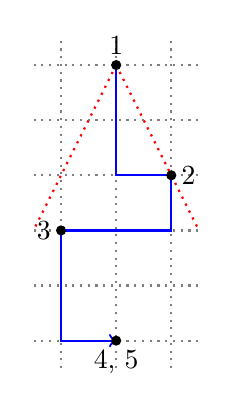
\begin{tikzpicture}[thick, scale=0.7]
      \draw[dotted, gray] (-1.5,-5.5) grid (1.5,0.5); % Dotted grid
      \draw[dotted, red] (0,0) -- (1.5,-3);
      \draw[dotted, red] (0,0) -- (-1.5,-3);
      \draw[blue,->] (0,0) -- (0,-2) -- (1,-2) -- (1,-3) -- (-1,-3) -- (-1,-5) -- (0,-5);
      \filldraw[black, thick] (0,0) circle (2pt) node[above] {1};
      \filldraw[black, thick] (1,-2) circle (2pt) node[right] {2};
      \filldraw[black, thick] (-1,-3) circle (2pt) node[left] {3};
      \filldraw[black, thick] (0,-5) circle (2pt) node[below] {4, 5};
  \end{tikzpicture}}
  \subfigure[Tip]{
  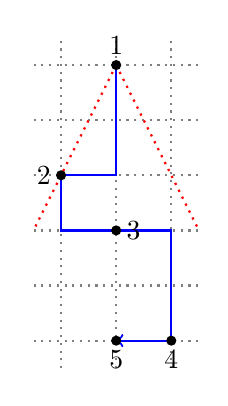
\begin{tikzpicture}[thick,scale=0.7]
      \draw[dotted, gray] (-1.5,-5.5) grid (1.5,0.5); % Dotted grid
      \draw[blue,->] (0,0) -- (0,-2) -- (-1,-2) -- (-1,-3) -- (0,-3) -- (1,-3) -- (1,-5) -- (0,-5);
      \draw[dotted, red] (0,0) -- (1.5,-3);
      \draw[dotted, red] (0,0) -- (-1.5,-3);
      \filldraw[black, thick] (0,0) circle (2pt) node[above] {1};
      \filldraw[black, thick] (-1,-2) circle (2pt) node[left] {2};
      \filldraw[black, thick] (0,-3) circle (2pt) node[right] {3};
      \filldraw[black, thick] (1,-5) circle (2pt) node[below] {4};
      \filldraw[black, thick] (0,-5) circle (2pt) node[below] {5};
  \end{tikzpicture}}
  \subfigure[Tip]{
  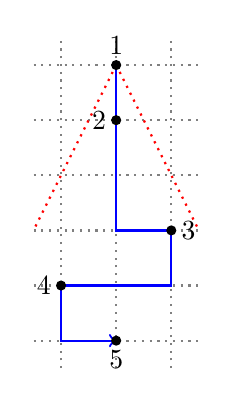
\begin{tikzpicture}[thick, scale=0.7]
      \draw[dotted, gray] (-1.5,-5.5) grid (1.5,0.5); % Dotted grid
      \draw[blue,->] (0,0) -- (0,-3) -- (1,-3) -- (1,-4) -- (-1,-4) -- (-1,-5) -- (0,-5);
      \draw[dotted, red] (0,0) -- (1.5,-3);
      \draw[dotted, red] (0,0) -- (-1.5,-3);
      \filldraw[black, thick] (0,0) circle (2pt) node[above] {1};
      \filldraw[black, thick] (0,-1) circle (2pt) node[left] {2};
      \filldraw[black, thick] (1,-3) circle (2pt) node[right] {3};
      \filldraw[black, thick] (-1,-4) circle (2pt) node[left] {4};
      \filldraw[black, thick] (-0,-5) circle (2pt) node[below] {5};
  \end{tikzpicture}}
  \subfigure[Tip]{
  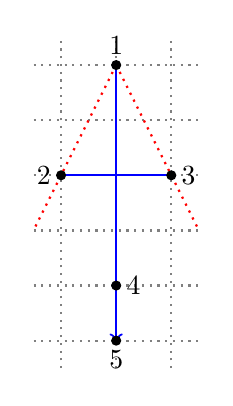
\begin{tikzpicture}[thick, scale=0.7]
      \draw[dotted, gray] (-1.5,-5.5) grid (1.5,0.5); % Dotted grid
      \draw[blue,->] (0,0) -- (0,-2) -- (-1,-2) -- (1,-2) -- (0,-2) -- (0,-4) -- (0,-5);
      \draw[dotted, red] (0,0) -- (1.5,-3);
      \draw[dotted, red] (0,0) -- (-1.5,-3);
      \filldraw[black, thick] (0,0) circle (2pt) node[above] {1};
      \filldraw[black, thick] (-1,-2) circle (2pt) node[left] {2};
      \filldraw[black, thick] (1,-2) circle (2pt) node[right] {3};
      \filldraw[black, thick] (0,-4) circle (2pt) node[right] {4};
      \filldraw[black, thick] (0,-5) circle (2pt) node[below] {5};
  \end{tikzpicture}}
  \subfigure[Stage]{
  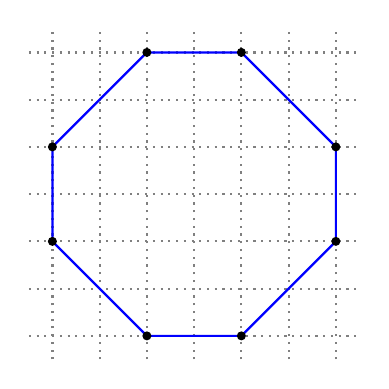
\begin{tikzpicture}[thick, scale=0.6]
      \draw[dotted, gray] (-2.5,-0.5) grid (4.5,6.5); % Dotted grid
      \draw[blue,-] (0,0) -- (2,0) -- (4,2) -- (4,4) -- (2,6) -- (0,6) -- (-2,4) -- (-2,2) -- (0,0);
      \filldraw[black] (0,0) circle (2pt);
      \filldraw[black] (2,0) circle (2pt);
      \filldraw[black] (4,2) circle (2pt);
      \filldraw[black] (4,4) circle (2pt);
      \filldraw[black] (2,6) circle (2pt);
      \filldraw[black] (0,6) circle (2pt);
      \filldraw[black] (-2,4) circle (2pt);
      \filldraw[black] (-2,2) circle (2pt);
  \end{tikzpicture}}
  \caption{Vier vordefinierte Pfade für das Zurückziehen der Messspitzen. Der Verfahrweg wird mit der Vergrößerung skaliert. Die Probe wird zyklisch verfahren.}
  \label{fig:pathmanip}
\end{figure}

Zunächst wird jedem Manipulator ein zufälliger Pfad zugewiesen, den er abfahren wird. Anschließend wird eine Maske eingezogen, die später für die Annotation verwendet wird.
Das System nimmt nun eine vordefinierte Anzahl von Bildern der eingestellten Szene auf. Für jedes Bild wird eine zufällige Konstellation von REM-Parametern aus einem vordefinierten Satz ausgewählt. Die Probe wird zwischen jedem Bild an eine andere Position bewegt. Dazu ist eine zyklische Bahn definiert und die Probe wird so ausgerichtet, dass sie auf dem Pfad eine möglichst große Variation der Probenstruktur abdeckt. Da die Spitzen während der Aufnahme der fünf Bilder ihre Position beibehalten, kann die zuvor erstellte Maske zur Markierung der Spitzenposition für alle Bilder der Szene verwendet werden.

\begin{figure}[h]
    \centering
    \subfigure[]{
    \includegraphics[width=.3\linewidth]{img/000.png}
    \label{fig:augimg0}
    }
    \subfigure[]{
    \includegraphics[width=.3\linewidth]{img/001.png}
    \label{fig:augimg1}
    }
    \subfigure[]{
    \includegraphics[width=.3\linewidth]{img/002.png}
    \label{fig:augimg2}
    }
    \subfigure[]{
    \includegraphics[width=.3\linewidth]{img/003.png}
    \label{fig:augimg3}
    }
    \subfigure[]{
    \includegraphics[width=.3\linewidth]{img/004.png}
    \label{fig:augimg4}
    }
    \caption{Eine Szene aufgenommen mit verschiedenen Parametern. Deutlich zu erkennen ist der Unterschied zwischen dem SE2 Detektor in (a), (c) und (e) und dem InLens Detektor in (b) und (d). Die Probenstruktur ist sehr unterschiedlich.}
    \label{fig:augimg}
\end{figure}
Dadurch reduziert sich der Aufwand für die nachfolgende Annotation auf ein Fünftel. Dieser Vorgang wird wiederholt, bis alle Spitzen die Endposition der ihnen zugewiesenen Pfade erreicht haben. Dann wird die nächst kleinere Vergrößerungsstufe (beginnend bei 50.000x, dann 25.000x, 10.000x und zuletzt 2.000x) verwendet und der Vorgang wiederholt.

Es ist wichtig, die zeitlichen Anforderungen dieses Prozesses zu berücksichtigen. Im Vorfeld wird viel Zeit darauf verwendet, die Nadeln in ihre Ausgangsposition zu bringen und die Parameter für ein scharfes Bild einzustellen. Beide Prozesse erfordern eine Reihe fein abgestimmter Einstellungen, die alle miteinander interagieren. Außerdem dauert ein einzelner Durchlauf der Routine etwa eine Stunde. Trotz dieser Herausforderungen stellt die automatisierte Bildaufnahme einen effizienten Ansatz dar, um eine große Anzahl von Bildern mit variablen Parametern zu erzeugen.

\begin{algorithm}[h!]
\begin{algorithmic}[1]
\caption{Routine für das automatische Einziehen der Bilder.}
\label{alg:Pseudocode}
\REQUIRE{Liste von Vergrößerungen: mags, Anzahl an Bildern pro Szene: count, Verwendete Abtastraten: srs, Verwendete Detektoren: dets, Zwei Arbeitsdistanzen: wds}
\ENSURE{Einen Datensatz an Bildern}
\FOR{mag \textbf{in} mags}
  \STATE controller.assignPattern()
  \COMMENT{Weise jedem Manipulator einen zufälligen Pfad zu}
  
  \FOR{$i \leftarrow 0$ \textbf{to} controller.patternLength()}
    \STATE sem.grabImage(mag, dt='SE2', sr='10', wds[0])
    \COMMENT{Ziehe ein Maskenbild ein.}
    \FOR{$j \leftarrow 0$ \textbf{to} count}
        \STATE wd, sr, dt $\leftarrow$ random(wds, srs, dts)
        \COMMENT{Wähle zufällige Mikroskop Parameter}
        \STATE sem.grabImage(mag, dt, sr, wd)
        \COMMENT{Ziehe ein Bild ein.}
        \STATE controller.moveStage()
        \COMMENT{Bewege die Probe.}
    \ENDFOR
    \STATE controller.restractStep()
    \COMMENT{Bewege die Manipulatoren}
  \ENDFOR
\ENDFOR
\end{algorithmic}
\end{algorithm}
\subsection{Ergebnis}
Bei einem Durchlauf der Routine, mit vier Vergrößerungsstufen, fünf Spitzenpositionen
und fünf Bildern pro Szene, werden insgesamt 100 Bilder und 20 Masken
erzeugt. Diese Routine wird sechsmal durchgeführt, jeweils mit verschiedenen
Ausgangspositionen der Spitzen und verschiedenen Positionen der Probe. Somit
ergeben sich insgesamt 600 Bilder und 100 zugehörige Masken.
\clearpage
\section{Daten Annotation}
\subsection{Segmentierung}
Bei der Erstellung der Annotation der Masken, wird bewusst auf polygonbasierte Werkzeuge verzichtet, da diese eine pixelgenaue Segmentierung erschweren. Daher wird Adobe Photoshop \cite{adobephotoshop} als Werkzeug der Wahl eingesetzt. Photoshop bietet eine Reihe von Werkzeugen, wie das \glqq Magnetic Lasso\grqq{} und \glqq Quick Select\grqq{}, die eine pixelgenaue Auswahl von Objekten erleichtern.

Um die Annotation zu vereinfachen und zu standardisieren, werden acht optisch und numerisch deutlich unterscheidbare Farben zur Markierung der Spitzen verwendet. Dabei wird darauf geachtet, dass den Spitzen aus einer bestimmten Himmelsrichtung immer die gleiche Farbe zugewiesen wird. Dies ermöglicht nicht nur die Unterscheidung der Instanzen, sondern gibt unter Berücksichtigung der Bildrotation auch Auskunft darüber, in welchem Manipulator die Spitze montiert ist. Nachdem alle Spitzen markiert sind, wird der restliche Bildbereich schwarz eingefärbt.

Um die Qualität der Annotationen sicherzustellen, wird mit Experten von Kleindiek definiert, welche Bereiche zu den Spitzen gehören und wie die Konturen zu zeichnen sind.

\begin{figure}[htbp]
    \centering
    \subfigure[Rohbild]{
    \includegraphics[width=0.45\linewidth]{img/drifttest_stop_017_0.png}
    }
    \subfigure[Maske]{
    \includegraphics[width=0.45\linewidth]{img/drifttest_stop_017.png}
    }
    \caption{Bild und zugehörige annotierte Maske. Die HEX-Farbwerte sind hier in die Spitzen eingezeichnet.}
    \label{fig:mask}
\end{figure}
Da Photoshop ursprünglich für die Bearbeitung und Verbesserung von Fotografien entwickelt wurde, treten trotz pixelgenauer Auswahl Probleme auf. Denn Photoshop erzeugt keine harten Kanten. Die Farben einiger Grenzpixel vermischen sich leicht.
Dies ist problematisch, da dadurch in den Masken Farben auftreten, die nicht den vordefinierten Farben entsprechen und somit zu Fehlern in der Weiterverarbeitung führen.

Versuche, dieses Problem durch nachträgliche Manipulation von Kontrast, Helligkeit und Sättigung zu beheben, waren nicht erfolgreich. Daher wurde ein Python-Skript zur Nachbearbeitung der annotierten Masken entwickelt.
Genutzt werden dazu die Python Bibliotheken von SciPy \cite{2020SciPy-NMeth}, Pillow \cite{clark2015pillow} und OpenCV \cite{opencv_library}.

Da für die Annotation numerisch gut unterscheidbare Farben gewählt wurden und da ein Pixel – definiert durch das Tupel (r, g, b) – auch als Vektor im dreidimensionalen Raum interpretiert werden kann, lässt sich für jedes Pixel, das von den acht definierten Farben abweicht, die Manhattan-Distanz berechnen und der Wert des Pixels auf den nächstgelegenen Wert setzen.
Auf diese Weise konnten alle Pixelfehler ohne Qualitätsverlust der Annotation beseitigt werden.

\subsection{Konvertierung in das COCO Datenformat}
Mehrere Schritte sind erforderlich, um die erstellten Bilder und annotierten Masken in das COCO-Datenformat zu konvertieren.

Zunächst muss der Datensatz in einen Trainings- und einen Validierungsteil aufgeteilt werden. Zu diesem Zweck werden zwei JSON-Dateien, train.json und val.json, erstellt. In diese Dateien müssen nun alle Klassen, Bilder und Annotationen eingetragen werden.

Um die erstellten Masken in das COCO Format zu übersetzen, müssen zunächst die eingefärbten Spitzen als Polygon dargestellt werden. Dazu werden die Umrisse der eingefärbten Bereiche extrahiert. Zweitens müssen die Bounding-Box-Werte aus den Grenzen des Polygons bestimmt werden. Drittens muss der vorderste Punkt der Spitze bestimmt werden, um den Keypoint zu markieren.
Um diese Aufgaben zu lösen, wird ein Ansatz adaptiert, der von Chris Eijgenstein in seinem Projekt image-to-coco-json-converter genutzt wurde \cite{chriscoco}. Dieser Ansatz verwendet die Python-Bibliotheken shapely \cite{shapely2007}, scikit-image \cite{van2014scikit} und Pillow \cite{clark2015pillow}, um die Konturen der Annotationen aus einem Maskenbild zu extrahieren. Dabei ist zu beachten, dass sich Spitzen überlappen können und somit in 2 Bereiche unterteilt werden. Die Kontur einer Spitzeninstanz wird mit skimage aus dem Bild extrahiert. Shapely stellt die Kontur als Polygon dar und berechnet die Parameter der Bounding Box.
Zur Markierung des Keypoint wird das Binärbild der Kontur mit OpenCV \cite{opencv_library} angezeigt und der Benutzer muss den vordersten Punkt der Spitze entsprechend markieren.
Um ein Maximum an Informationen zu erhalten, werden die acht Spitzen während des gesamten Prozesses als getrennte Klassen behandelt.

Eine Herausforderung besteht darin, eine annotierte Maske mit allen zugehörigen Bildern zu verknüpfen, da sie nach der Konvertierung in das COCO-Format nur über eine ID referenziert wird und nicht über den Dateinamen, wie es bei der Erstellung der Bilder der Fall ist. Zu diesem Zweck werden bereits konvertierte Masken mit Verweis auf ihren Dateinamen zwischengespeichert. Bei nachfolgenden Bildern wird geprüft, ob die zugehörige Maske bereits konvertiert wurde. Falls bereits eine Annotation in COCO-Format vorhanden ist, müssen die Werte \glqq id\grqq{} und \glqq image\_id\grqq{} entsprechend angepasst werden. Dabei ist immer auf die korrekte Nummerierung zu achten, da es sonst zu Konflikten kommen kann.
Es ist notwendig, dass alle anderen Parameter des COCO-Formats ebenfalls korrekt gesetzt sind. Diese sind jedoch trivialer und werden daher hier nicht weiter erläutert.

\subsubsection{Konvertierungsskript}
Zur Automatisierung und Vereinfachung des Konvertierungsprozesses, wird ein spezielles Python-Skript entwickelt. Dieses Skript kann von der Kommandozeile aus aufgerufen werden und ermöglicht es, den gesamten Konvertierungsprozess mit einem einzigen Befehl auszuführen. Es nimmt den Pfad zu dem Ordner als Eingabe und führt dann die Konvertierung durch.
\begin{figure}[h]
\centering
\begin{minipage}{0.4\linewidth}
\dirtree{%
.1 /.
.2 dataset.
.3 images.
.4 image0.tif.
.4 ....
.3 masks.
.4 mask0.png.
.4 ....
.2 dataset-coco.
.3 images.
.4 image0.tif.
.4 ....
.3 annotations.
.4 train.json.
.4 val.json.
}
\end{minipage}
    \caption{Darstellung der Verzeichnisstruktur des Datensatzes vor und nach der Konvertierung. Die Anzahl der erstellten Ordner hängt von der Wahl der Parameter des Konvertierungsskripts ab.}
    \label{fig:folderstruc}
\end{figure}

Jeder erzeugte Datensatz wird in einem separaten Ordner gespeichert, sodass er sofort für Trainingszwecke verwendet werden kann. Die benötigte und erstellte Ordnerstruktur ist in \ref{fig:folderstruc} dargestellt.

Das Besondere an diesem Skript ist seine Flexibilität. Es erlaubt die Spezifikation beliebiger Parameterkombinationen und erzeugt entsprechend die gewünschten Datensätze. Dies ermöglicht die Erstellung maßgeschneiderter Datensätze, die auf spezifische Anforderungen und Anwendungsszenarien zugeschnitten sind. Darüber hinaus ist das Skript einfach zu verstehen und zu warten, was zukünftige Anpassungen und Erweiterungen erleichtert.
Die verfügbaren Skript-Parameter sind in Abbildung \ref{fig:param} aufgelistet.
\begin{figure}
    \centering
\begin{center}
\setlist{noitemsep}
\begin{description}
\item[\texttt{-dataset}] Pfad zum Datensatz (z.B. /home/user/dataset)
\item[\texttt{-split}] Aufteilungsverhältnis Training/Validierung (z.B. 0.8)
\item[\texttt{-coco}] Konvertierung in das COCO-Datenformat
\item[\texttt{-yolo}] Konvertierung in das YOLO-Datenformat
\item[\texttt{-oc}] Verwendung einer einzigen Klasse für alle Spitzen
\item[\texttt{-ib}] Einbeziehung des Hintergrunds für semantische/panoptische Segmentierung
\item[\texttt{-kp}] Einbeziehung der Koordinaten der Schlüsselpunkte
\item[\texttt{-mi}] Verwendung einer Maske für mehrere Bilder
\end{description}
\end{center}
    \caption{Skript-Parameter für die Konvertierung von Datensätzen.}
    \label{fig:param}
\end{figure}
% Ein Beispiel für die Verwendung des Skripts in der Kommandozeile könnte wie folgt aussehen:
% \begin{algorithmic}[htbp]
%     \STATE \text{\$ python convert\_dataset.py -dataset ./50img -split 0.9 -coco -oc -kp}
% \end{algorithmic}
% Dieser Befehl erzeugt aus den Bildern und Masken zwei Datensätze im COCO-Format: einen, in dem alle Spitzen als eine Klasse behandelt werden, und einen, in dem jede Spitze einer eigenen Klasse zugeordnet wird.
% Der Datensatz integriert die Koordinaten der Schlüsselpunkte. Diese müssen für jede Maske zur Laufzeit des Skripts markiert werden. Der Datensatz wird in einen Trainings- und einen Validierungsdatensatz aufgeteilt, wobei 90\% der Daten für das Training und 10\% für die Validierung verwendet werden.
\section{Datensätze}
Um die erforderlichen Skripte zu entwickeln sowie die Entwicklungsumgebung einzurichten und zu testen, wurde eine Reihe von Datensätzen erstellt. Eine tabellarische Übersicht aller Datensätze ist in der Tabelle \ref{tab:datasets} zu finden.
Die Benennung der Datensätze ist intuitiv und natürlich. Der erste Teil des Namens beschreibt die Anzahl der Bilder. Verschiedene Suffixe werden angehängt, um Informationen darüber zu liefern, wie die Masken annotiert sind. Beispielweise steht das Suffix \glqq -oc\grqq{}für \glqq one class\grqq{} (eine Klasse). Die Klassen des Datensatzes sind zusammengefasst. Die Spitzen werden also nicht nach ihrer Richtung unterschieden.

Der Datensatz \glqq 50img\grqq{} enthält 50 Bilder und Masken aus realen Einsatzszenarien. Es diente zur Überprüfung der Annotationsmethode und der Konvertierung in das COCO-Format. Er wurde auch verwendet, um die Entwicklungsumgebung so zu konfigurieren, dass das Training von Mask R-CNN später schnell auf einem großen Datensatz durchgeführt werden kann. 
Der Datensatz \glqq 600img\_1x5\grqq{} enthält 600 Bilder, wobei eine Maske auf fünf Bilder passt, und wurde mit der entwickelten automatischen Bildaufnahmemethode erstellt. Er wird später einen Großteil der Trainingsdaten darstellen.
\glqq 617img\_batch1\grqq{} enthält 100 von insgesamt 617 sorgfältig ausgewählten Bildern aus realen Einsätzen. Sie repräsentieren eine Vielzahl von Szenarien und sollen als Grundlage für eine genaue Darstellung dienen.

Alle Bilder und Masken der oben genannten Datensätze sind in dem Datensatz \glqq 750img\_merged\grqq{} zusammengefasst. Er besteht somit aus 600 Bildern, die durch das Skript erzeugt wurden, und 150 Bildern, die aus realen Einsätzen stammen. Nach einer genaueren Analyse des Datensatzes stellte sich heraus, dass Spitzen aus verschiedenen Richtungen unterschiedlich häufig in den Bildern vertreten sind. Dies wird auf die 150 Bilder aus realen Einsätzen zurückgeführt. Dargestellt ist die Verteilung in Abbildung \ref{fig:instpclass}. Es zeigt sich, dass insbesondere die Spitzen fünf (Süd) und sechs (Süd-West) seltener im Einsatz sind. Dennoch wird der Datensatz für das Training von Mask R-CNN verwendet und in der Evaluierung wird untersucht, inwieweit sich dieses Ungleichgewicht auf die Leistungsfähigkeit des Modells auswirkt.
\begin{table}[h]
\begin{adjustbox}{width=\columnwidth,center}
\begin{tabular}{llllll}
\toprule
\textbf{Name} & \textbf{Bildanzahl} & \textbf{Augmentation} & \textbf{Klassen} & \textbf{Entwicklung} & \textbf{Training} \\
\midrule
50img         & 50                  & Nein                     & 8                 & Ja                    & Nein              \\
50img-oc      & 50                  & Nein                   & 1                 & Ja                    & Nein              \\
600img\_1x5        & 600                 & Ja                     & 8                 & Ja                    & Nein              \\
617img\_batch1     & 100                 & Nein                   & 8                 & Nein                  & Nein              \\
750img\_merged        & 750                 & Teils                     & 8                 & Nein                  & Ja                \\
750img\_merged-oc     & 750                 & Teils                     & 1                 & Nein                  & Ja                \\
\bottomrule
\end{tabular}
\end{adjustbox}
\caption{Zusammenfassung der Datensätze. Alle Datensätze haben ein Train-Val-Verhältnis von 0.9}
\label{tab:datasets}
\end{table}

% \begin{figure}[htbp]
%     \centering
%     \begin{tikzpicture}
%         \begin{axis}[
%             ybar,
%             bar width=0.5cm,
%             width=12cm,
%             height=8cm,
%             xlabel={Tip},
%             ylabel={Anzahl},
%             symbolic x coords={tip1, tip2, tip3, tip4, tip5, tip6, tip7, tip8},
%             enlargelimits=0.15,
%             legend style={at={(0.5,-0.15)},
%                 anchor=north,legend columns=-1},
%             xtick=data,
%             nodes near coords,
%             nodes near coords align={vertical},
%             ymin=0
%         ]
%         \addplot coordinates {(tip1, 35) (tip2, 14) (tip3, 32) (tip4, 19) (tip5, 34) (tip6, 12) (tip7, 32) (tip8, 15)};
%         \addplot coordinates {(tip1, 528) (tip2, 556) (tip3, 482) (tip4, 406) (tip5, 293) (tip6, 293) (tip7, 589) (tip8, 503)};
%         \legend{50img, 750img\_merged}
%         \end{axis}
%     \end{tikzpicture}
%     \caption{Verteilung der Klassen im Entwicklungs- und Trainingsdatensatz. 50img enthält 193 Instanzen. 750img\_merged enthält 3650 Instanzen. Es fällt auf, dass insbesondere die Klassen tip5 und tip6 in den Daten unterrepräsentiert sind.}
%     \label{fig:my_bar_chart}
% \end{figure}
\begin{figure}[h]
    \centering
    \includegraphics[trim={0.2cm 0.2cm 0.2cm 0.2cm}, clip]{img/eval/inst_per_class.png}
    \caption{Anzahl der Instanzen jeder Spitzenklasse von \glqq 750img\_merged\grqq{}. Dies ermöglicht einen Vergleich zwischen den Klassenverteilungen in den Trainings- und Validierungsdaten.}
    \label{fig:instpclass}
\end{figure}

\clearpage
\section{Implementierung und Training der Modelle}
\subsection{Entwicklungsumgebung}
Für diese Entwicklung wird ein System mit Ubuntu in der Version 22.04 verwendet. Die effiziente Nutzung der zugrunde liegenden Grafikkarte vom Typ \glqq Nvidia GTX 1080\grqq{} wird durch die Installation von CUDA 11.8 erreicht, einer von Nvidia entwickelten parallelen Berechnungsplattform und Anwendungsprogrammierschnittstelle (API). CUDA ermöglicht es Entwicklern, Software zu schreiben, die die Hardwarebeschleunigung für rechenintensive Anwendungen nutzt, insbesondere in den Bereichen maschinelles Lernen und Datenverarbeitung \cite{cuda}.

Für die Entwicklung der Netze wird PyTorch in der Version 2.0.1 zusammen mit torchvision-0.15.1 installiert. PyTorch ist ein Open-Source-Maschinelearning-Framework, das die schnelle Entwicklung von Deep Learning-Algorithmen ermöglicht. Es bietet sowohl flexible als auch effiziente Implementierungen von verschiedenen Arten von neuronalen Netzen und anderen maschinellen Lern-Algorithmen \cite{NEURIPS2019_9015}. Die entsprechenden Versionen wurden vorab für CUDA 11.8 kompiliert, um das Training auf der Grafikkarte zu ermöglichen und damit zu beschleunigen.

Für das Training der Netze wird Detectron2 verwendet. Da für diese spezielle Systemkonfiguration keine vorkompilierte Version von Detectron2 verfügbar ist, wird sie aus dem Quellcode erstellt.

Die oben beschriebene Entwicklungsumgebung wird hauptsächlich für die Vor- und Nachverarbeitung der Daten sowie für die Implementierung und das Debugging des Mask R-CNN Modells verwendet. Da diese Umgebung jedoch nicht die erforderliche Rechenleistung für ein schnelles und effizientes Training des Modells bietet, wird das Training selbst in einer Cloud-basierten Umgebung, konkret auf Google Colab, durchgeführt.

Google Colab ist eine Cloud-Service-Plattform, die GPU-Ressourcen für maschinelles Lernen und datenwissenschaftliche Forschung zur Verfügung stellt \cite{google-colab}.
Für das Training wird eine Instanz mit einer Nvidia V100 Grafikkarte ausgewählt. Die Nvidia V100 ist eine Hochleistungs-GPU, die speziell für maschinelles Lernen und rechenintensive Anwendungen entwickelt wurde. Sie bietet eine erhebliche Beschleunigung im Vergleich zu Consumer-Grafikkarten und ist mit 16 Gigabyte Grafikspeicher ideal für das Training von Deep Learning Modellen geeignet.
In dieser Google Colab Umgebung ist es notwendig, Detectron2 zu installieren. Durch den Einsatz von Google Colab kann trotz der Hardwarebeschränkungen der lokalen Entwicklungsumgebung ein effizientes Training des Modells erreicht werden.
\subsection{Implementierung von Mask R-CNN}
Der sogenannte \glqq Model Zoo\grqq{} von Detectron2, eine Sammlung von vorgefertigten Modellen und Konfigurationen für verschiedene Algorithmen und deren Varianten enthält auch verschiedene Implementierungen von Mask R-CNN und Keypoint R-CNN, die als Ausgangspunkt für das in dieser Arbeit verwendete Modell dienten.

Mask R-CNN wurde aufgrund seiner Modularität ausgewählt. Es kann schnell angepasst werden, um Objektdetektion, Segmentierung und Keypoint-Erkennung durchzuführen, andere Modellarchitekturen bieten diese Flexibilität nicht.

Von besonderem Interesse sind die verschiedenen Backbone-Architekturen, die im Model Zoo von Detectron2 zur Verfügung stehen. Es werden die Backbones R50-FPN, R50-DC5, R101-FPN und R101-DC5 verwendet.
Eine detaillierte Erläuterung der Backbones findet sich in Kapitel \ref{sec:backbone}.

% , hier jedoch eine kurze Zusammenfassung.
% ResNet-50 (R50) und ResNet-101 (R101) sind Varianten des ResNet-Modells, die eine effiziente Lösung für das Problem des verschwindenden Gradienten in tiefen neuronalen Netzen bieten. FPN steht für Feature Pyramid Network, eine Netzarchitektur, die Informationen aus mehreren Extraktionsebenen verwendet, um die Genauigkeit der Objekterkennung zu verbessern. DC5 bezeichnet eine Konfiguration, bei der alle 3x3-Convolutions in der C5-Stufe von ResNet durch 3x3-Dilated-Convolutions ersetzt werden.

\begin{figure}[h]
    \centering
    \includegraphics[width=0.8\linewidth, clip, trim={0 4cm 10cm 0.5cm}]{img/model_arch.png}
    \captionsource{Die verwendete Mask R-CNN Architektur, der Keypoint-Zweig wird angefügt. Die Keypoints werden als eine One-Hot Maske ausgegeben.}{Modifiziert übernommen von He \textit{et al.} \cite{He_2017_ICCV}}
    \label{fig:modelarch}
\end{figure}
Da das Modell sowohl Schlüsselpunkte als auch Segmentierungsmasken ausgeben soll, werden die entsprechenden Konfigurationen von Mask R-CNN und Keypoint R-CNN zusammengefasst, die Architektur ist in Abbildung \ref{fig:modelarch} dargestellt. Auf diese Weise können die Vorteile beider Modelltypen genutzt werden und das Modell erzeugt beide Ausgaben gleichzeitig.

Die Konfigurationen werden entsprechend den spezifischen Anforderungen dieser Arbeit angepasst, wobei die Details der Anpassungen im Abschnitt \ref{sec:hyperp} über die Einstellung der Hyperparameter näher beschrieben werden. Mit diesen Einstellungen konnte ein maßgeschneidertes Mask R-CNN Modell entwickelt werden, das speziell für die Aufgabe der Lokalisierung von Messspitzen im REM geeignet ist.
\subsection{Verwendung und Anpassung der vortrainierten Gewichte}
%Durch die Verwendung vortrainierter Gewichte kann das Modell effizienter trainiert werden. Dies bedeutet, dass das Modell auf den bereits gelernten Eigenschaften der vortrainierten Gewichte aufbaut, was den Trainingsprozess beschleunigt und eine bessere Leistung des Modells ermöglicht, als wenn das Modell von Grund auf neu trainiert würde.
Für diese Arbeit werden verschiedene vortrainierte Modelle aus dem Detectron2 Model Zoo verwendet, aufgelistet sind diese in Tabelle \ref{tab:modelle}.
Diese Modelle wurden ursprünglich auf dem COCO \glqq train2017\grqq{} Datensatz trainiert, einem großen und vielfältigen Datensatz zur Objekterkennung, Segmentierung und Keypoint-Erkennung \cite{coco}.

Da das Modell zur Spitzenerkennung beide Fähigkeiten – Masken- und Keypoint-Vorhersage – beherrschen soll, werden die vortrainierten Gewichte des Keypoint-Zweiges aus den Keypoint R-CNN-Modellen extrahiert und mit den Parametern des entsprechenden Mask R-CNN-Modells mithilfe eines Python-Skripts kombiniert. Dies ermöglicht die Erstellung eines vortrainierten Modells, das sowohl die bereits erlernten Fähigkeiten zur Maskengenerierung als auch zur Keypoint-Erkennung besitzt.

\begin{table}[h]
\centering
\begin{tabular}{lll}
\toprule
\textbf{Name} & \textbf{Backbone} & \textbf{LR Schedule} \\
\midrule
Mask R-CNN & R50-DC5 & 3x \\
Mask R-CNN & R50-FPN & 3x \\
Keypoint R-CNN & R50-FPN & 3x \\
Mask R-CNN & R101-FPN & 3x \\
Mask R-CNN & R101-DC5 & 3x \\
Keypoint R-CNN & R101-FPN & 3x \\
\bottomrule
\end{tabular}
\caption{Genutzte vortrainierte Modelle aus dem Detectron2 Model Zoo.}
\label{tab:modelle}
\end{table}
Es ist jedoch anzumerken, dass für die DC5 Varianten der Backbones keine vortrainierten Gewichte für den Keypoint-Zweig zur Verfügung stehen. In diesem Fall wird das Modell nur mit den verfügbaren Mask R-CNN Gewichten trainiert.

Um den vollen Nutzen aus den vortrainierten Gewichten zu ziehen, wird ein spezielles Trainingsschema verwendet. In einer ersten Phase wird das Backbone des Modells \glqq eingefroren\grqq{}, das heißt, es werden keine Gradienten berechnet und die Gewichte werden nicht aktualisiert. Dadurch kann der Maskenkopf des Modells lernen, die Positionen und Konturen der Spitzen auf Grundlage der bereits gelernten Merkmale des Backbone zu rekonstruieren.
In der zweiten Phase des Trainingsprozesses wird das gesamte Modell einschließlich des Backbones auf dem spezifischen Datensatz trainiert. Dieser Schritt stellt sicher, dass das Modell genau an die spezifische Aufgabe angepasst ist. Zur Unterstützung dieses zweiphasigen Trainingsprozesses wird eine speziell angepasste Lernrate verwendet, die den Fortschritt des Modells in beiden Phasen effektiv steuert. Die entwickelte Lernrate ist in Abbildung \ref{fig:lr} zu sehen.
\subsection{Wahl der Hyperparameter}
\label{sec:hyperp}
In Detectron2 wird für das Training auf acht GPUs eine Lernrate von 0,02 verwendet. Die lineare Skalierungsregel von Goyal \textit{et al.} \cite{1706.02677} besagt, dass die Lernrate proportional zur Anzahl der GPUs angepasst werden sollte. Daher wird die anfängliche Lernrate für das Training auf einer einzelnen GPU auf 0,002 reduziert.

Für den Optimierer wird ein Momentum-Wert von 0,9 festgelegt. Dies hilft, den Trainingsprozess in die richtige Richtung zu beschleunigen. Eine Gewichtsabnahme von 0,0001 wird verwendet, und reguliert  die Überanpassung.
16 Bilder pro Batch sind die optimale Anzahl, um die Leistung der Nvidia V100 GPU voll auszunutzen, ohne sie zu überlasten. Dies trägt zu einer effizienten Nutzung der Hardware-Ressourcen bei, ohne die Qualität des Trainings zu beeinträchtigen.

\begin{figure}[h]
    \centering
    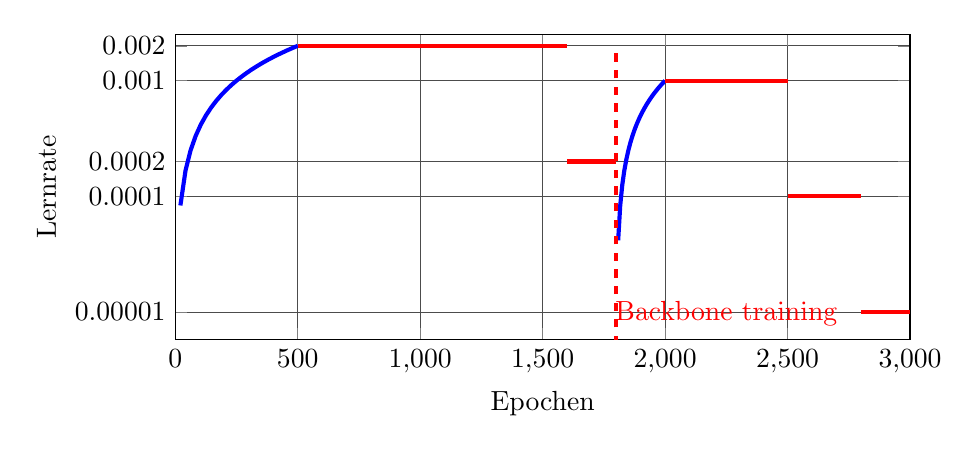
\begin{tikzpicture}
        \begin{axis}[
            xlabel=Epochen,
            ylabel=Lernrate,
            xmin=0, xmax=3000,
            ymin=0, ymax=0.0025,
            height=0.45\textwidth,
            width=0.9\textwidth,
            ymode=log, % Set the y-axis to log scale
            xtick={0,500,1000,1500,2000,2500,3000},
            ytick={0.00001, 0.0001, 0.0002, 0.001, 0.002},
            yticklabels={0.00001, 0.0001, 0.0002, 0.001, 0.002}, % Set the tick labels
            ytickten={-5, -4, -3, -2, -1}, % Specify the power of 10 for the ticks
            grid=both,
            grid style={line width=.3pt, draw=black!70},
        ]
            % First linear segment
            \addplot[domain=0:500, blue, line width=1.5pt] {0.002*x/500};
            
            % Constant segment
            \addplot[domain=500:1600, red, line width=1.5pt] {0.002};
            
            % Second linear segment
            \addplot[domain=1600:1800, red, line width=1.5pt] {0.0002};
            
            % Third linear segment
            \addplot[domain=1800:2000, blue, line width=1.5pt] {0.001*(x-1800)/200};
            
            % Constant segment
            \addplot[domain=2000:2500, red, line width=1.5pt] {0.001};
            
            % Fourth linear segment
            \addplot[domain=2500:2800, red, line width=1.5pt] {0.0001};
            
            % Fifth linear segment
            \addplot[domain=2800:3000, red, line width=1.5pt] {0.00001};

            \draw [red, dashed, line width=1.5pt] (axis cs:1800, 0.0000001) -- (axis cs:1800, 0.002);
            \node[anchor=north, red] at (axis cs:2250, 0.000015) {Backbone training};
        \end{axis}
    \end{tikzpicture}
    \caption{Der Verlauf der Lernrate über die Epochen, logarithmisch dargestellt. Lernrate der Aufwärmepochen in Blau, konstante Lernrate in Rot.}
    \label{fig:lr}
\end{figure}
Die Modelle werden für 3000 Epochen trainiert. Während der Entwicklung und Erprobung hat sich diese Zahl als optimal für ein ausgewogenes Verhältnis zwischen Modellleistung und Trainingszeit erwiesen.
Die ersten 500 Epochen des Trainings dienen als Aufwärmphase. In dieser Phase wird die Lernrate schrittweise linear auf die eingestellte Lernrate erhöht. Liu \textit{et al.} haben gezeigt, dass dieser Vorgang dazu beitragen kann, das Modell besser auf das Training vorzubereiten und Instabilitäten zu Beginn des Trainings zu vermeiden \cite{1908.03265}.

In den ersten 1800 Epochen werden die Masken und der Keypoint-Kopf trainiert, während das Backbone-Modell eingefroren bleibt. Die folgenden 1200 Epochen dienen der Feinabstimmung des gesamten Modells, einschließlich des Backbones. Diese zweite Trainingsphase beginnt wieder mit einer Aufwärmphase von 200 Epochen.

Die Lernrate wird während des Trainings in festgelegten Schritten abgestuft und reduziert, einerseits um die Modellkonvergenz zu fördern und andererseits ein Überspringen des globalen Minimums zu verhindern. Diese Anpassung ermöglicht eine anfänglich breitere Exploration des Lösungsraums und eine anschließende feinere Suche, wenn sich das Modell der optimalen Lösung nähert. Die entwickelte Strategie in Abbildung \ref{fig:lr} dargestellt.
\subsection{Erweiterung der Modelle: Richtungsvorhersage}
In einem weiteren Schritt werden die beiden Modellvarianten, die die beste Leistung bei der Erkennung von Spitzen aus allen Richtungen zeigen, erweitert. Dazu werden sie modifiziert und auf dem Datensatz \glqq 750\_merged\grqq{} trainiert. Die Spitzen werden nun nicht nur allgemein, sondern speziell nach ihrer Richtung unterschieden. Dahinter steht die Annahme, dass ein Modell, das in der Lage ist, Spitzen aus allen Richtungen zu erkennen, auch in der Lage sein könnte, diese Spitzen anhand ihrer spezifischen Position zu unterscheiden. Dies würde eine wesentliche Verbesserung für die automatisierte Steuerung darstellen, da eine nachträgliche Zuordnung der Segmentierung und der Schlüsselpunkte zur richtigen Spitze nicht mehr erforderlich wäre.

Es ist jedoch zu berücksichtigen, dass durch die spezifische Klassifizierung der Spitzen für jede Klasse insgesamt weniger Trainingsbilder zur Verfügung stehen. In einem ausgewogenen Datensatz führt dies zu einer Reduktion der Datenmenge auf ein Achtel pro Klasse. Dies stellt eine zusätzliche Herausforderung dar, da das Modell nun feinere Unterscheidungen treffen muss, während die Anzahl der Trainingsbeispiele pro Klasse reduziert wird.

Trotz der feineren Unterscheidung der Spitzen könnte die Aufgabe aus einer anderen Perspektive einfacher sein.
Da die Spitzen annähernd die gleichen Eigenschaften haben und sich hauptsächlich in ihrer Ausrichtung unterscheiden, muss jede der acht Masken Zweige des Modells nur eine der acht möglichen Darstellungen lernen. Da die auf eine Klasse trainierten Modelle bereits die Merkmale der Spitzen gelernt haben, werden die vortrainierten Backbones als Basis für die erweiterten Modelle verwendet. Die Masken-Zweige von Mask R-CNN werden von Grund auf neu trainiert.

Eine sorgfältige Bewertung der Leistung der Modelle ist entscheidend, um das Verhalten der Vorhersagen zu bestimmen, wenn das Modell auf diese Weise trainiert wird.
\chapter{Evaluation}
In diesem Kapitel liegt der Schwerpunkt auf der Evaluierung der im Rahmen dieser Arbeit entwickelten Modelle und Methoden.
Besonderes Augenmerk wird auf die Keypoint-Erkennung gelegt. Diese Technologie hat das Potenzial, revolutionäre Veränderungen in verschiedenen Anwendungsbereichen, insbesondere in automatisierten Prozessen, zu bewirken. Dies erfordert jedoch ein hohes Maß an Genauigkeit und Zuverlässigkeit. Daher wird die Genauigkeit der Modellvorhersagen systematisch analysiert, um ein klares Bild von der Zuverlässigkeit der Modelle zu erhalten und mögliche Schwachstellen aufzudecken.

Das Hauptziel dieses Kapitels ist es, zu verstehen, wie sich die Wahl des Backbones und der Hyperparameter auf die Leistung der Modelle auswirkt.
Da der Einsatz von Deep Learning für diese spezielle Aufgabenstellung ein neuer Ansatz ist und keine direkten Vergleichswerte vorliegen, ist es umso wichtiger, die vielversprechenden Möglichkeiten, aber auch die potenziellen Probleme zu diskutieren und zu bewerten.

Die Evaluierung ist in mehrere Teile gegliedert, beginnend mit der Definition der Evaluierungsmetriken, gefolgt von einer ausführlichen Evaluation auf dem Validierungsdatensatz. Diese beinhaltet die Ergebnisse der Segmentierung und der Keypoint-Vorhersage. Anschließend wird eine Analyse der fehlerhaften Vorhersagen durchgeführt, bevor die Vorhersagen in Bezug auf die Richtung der Spitze betrachtet werden. Der Abschnitt endet mit einer visuellen Überprüfung der Ergebnisse, um eine visuelle Beurteilung der Modellleistung zu ermöglichen.
\section{Evaluationsmetriken}
Zur Bewertung der in dieser Arbeit entwickelten Modelle werden verschiedene Metriken verwendet. Besonders betrachtet wird jedoch die $\text{AP}^{IoU=.75}$ und $\text{AP}^{OKS=.75}$. Diese strengen Varianten der AP erfordern einen IoU- und OKS-Wert von mehr als 0,75. Das bedeutet, dass nur die Vorhersagen als korrekt angesehen werden, die eine hohe Übereinstimmung mit den tatsächlichen Spitzen aufweisen.
Dies ist in unserer Anwendung besonders wichtig, da wir eine sehr genaue Lokalisierung und Erkennung der Spitzen anstreben. Eine niedrige $\text{AP}^{.75}$ würde auf viele Fehlentscheidungen des Modells hindeuten und könnte bei der Anwendung in automatisierten Prozessen zu Problemen führen. Daher streben wir einen hohen $\text{AP}^{IoU=.75}$ an, um die Zuverlässigkeit und Genauigkeit unserer Modelle zu gewährleisten.

Besonderes Augenmerk ist auch auf die Falsch-Negativ- und Falsch-Positiv-Raten zu richten. Eine Falsch-Positiv-Erkennung, bei der das Modell eine Spitze erkennt, wo keine ist, kann später zu einer Fehlsteuerung und damit zu großen Schäden führen. Dieser Fehlertyp ist daher unbedingt zu vermeiden. 
Ähnlich problematisch sind Falsch-Negativ-Erkennungen, bei denen das Modell eine vorhandene Spitze nicht erkennt. Dies kann insbesondere dann zu Problemen führen, wenn mehrere Spitzen dicht beieinander liegen und diese bewegt werden sollen. Um einen sicheren Betrieb zu gewährleisten, müssen dem System stets korrekte Informationen über die Position der Spitzen zur Verfügung stehen.
% \begin{figure}[htbp]
%     \centering
%     \includegraphics{img/eval/bboxap75.png}
%     \caption{AP der Bounding Box Vorhersage bei einem IoU-Wert von 0,75 für die verschiedenen Backbones während der Trainingsepisoden. Es ist zu erkennen, dass die AP nach ca. 1800 Epochen konvergiert, aber eine weitere Steigerung erfährt, sobald das Backbone-Training aktiviert wird. Diese Grafik zeigt die Entwicklung der Modellleistung während des Trainingsprozesses.}
%     \label{tab:bboxap75}
% \end{figure}

% \begin{table}[htbp]
% \centering
% \begin{tabular}{lrrr}
% \toprule
% Backbone & $\text{AP}$ & $\text{AP}^{IoU=.5}$ & $\text{AP}^{IoU=.75}$\\
% \midrule
% ResNet-50-FPN & 71.84 & 89.79 & 83.48 \\
% ResNet-50-C5-dilated & \textbf{77.21} & \textbf{93.65} & \textbf{86.11}\\
% ResNet-101-FPN & 75.13 & 92.71 & 85.39\\
% ResNet-101-DC5 & 77.85 & 94.44 & 87.47\\
% \bottomrule
% \end{tabular}
% \caption{AP Werte der Bounding-Box-Vorhersage, bei unterschiedlichen IoU Werten für die verschiedenen Modellvarianten. Mittelwert der letzten 200 Epochen.}
% \label{tab:bboxap}
% \end{table}
\section{Auswertung auf dem Validierungsdatensatz}
\begin{figure}[h]
    \centering
    \includegraphics[]{img/eval/total_loss.png}
    \caption{Gesamter Fehler der Modelle über die Trainingsepochen. Bei Iteration 1800 beginnt das training des Backbones.}
    \label{fig:loss}
\end{figure}
Die Abbildung \ref{fig:loss} zeigt den Gesamtfehler der trainierten Netze über die Epochen. Sie zeigt eine stabile Konvergenz aller Modelle ohne signifikante Sprünge, mit Ausnahme eines vorübergehenden Fehleranstiegs nach Iteration 1800, als das Training des Backbones zur Verfeinerung der Merkmalsextraktion beginnt. Die Kurven der verschiedenen Modelle überlagern sich, was auf ein ähnliches Lernverhalten hindeutet.
\clearpage
\subsection{Ergebnisse der Segmentierung}
\begin{table}[htbp]
\centering
\begin{tabular}{lrrr}
\toprule
Backbone & $\text{AP}$ & $\text{AP}^{IoU=.5}$ & $\text{AP}^{IoU=.75}$\\
\midrule
ResNet-50-FPN & 47.80 & 84.68 & 46.08 \\
ResNet-50-DC5 & 53.92 & \textbf{89.22} & \textbf{60.23}\\
ResNet-101-FPN & 50.39 & 88.62 & 51.01\\
ResNet-101-DC5 & \textbf{54.33} & 89.05 & 59.24\\
\bottomrule
\end{tabular}
\caption{Mittelwert der letzten 200 Epochen von $\text{AP}$, $\text{AP}^{IoU=.5}$, $\text{AP}^{IoU=.75}$ der Segmentierung für die verschiedenen Modelle.}
\label{tab:segap75}
\end{table}
\begin{figure}[h]
    \centering
    \includegraphics[trim={.3cm .25cm .2cm 1cm}, clip]{img/eval/segap75.png}
    \caption{Entwicklung der $\text{AP}^{IoU=.75}$ für die verschiedenen Backbones während der Trainingsepisoden.}
    \label{fig:segap75}
\end{figure}
Die AP-Werte der Segmentierung für verschiedene IoU-Werte, aufgeschlüsselt nach verschiedenen Backbone-Varianten sind in Tabelle \ref{tab:segap75} dargestellt. Bei den ResNet-50-Backbones ist ein Anstieg der AP um ca. fünf Prozent beim Wechsel von FPN zu DC5 zu beobachten. Dieser Trend ist bei allen AP-Varianten zu beobachten. Ähnliche Verbesserungen zeigen sich auch beim Wechsel von FPN zu DC5 in den ResNet-101-Backbones, insbesondere bei der strengen Metrik $\text{AP}^{IoU=.75}$, wo ein Anstieg von über acht Prozent gemessen wird. Auffällig ist, dass die Genauigkeit der Segmentierung zwischen den Netzwerken ResNet-50-DC5 und ResNet-101-DC5 nur einen Unterschied von weniger als einem Punkt aufweist.

Aus Abbildung \ref{fig:segap75} wird deutlich, dass die DC5-Varianten der Netze bereits nach 50 Epochen einen Trainingseffekt aufweisen. Im Gegensatz zur FPN-Variante, die erst nach 200 Epochen Vorhersagen liefert.  Über den gesamten Trainingszeitraum erreichen die DC5-Varianten eine höhere $\text{AP}^{IoU=.75}$ als die FPN-Varianten. Eine erkennbare Konvergenz aller Netze tritt nach 1800 Epochen auf. Die Aktivierung des Backbone-Trainings führt jedoch zu einem weiteren Anstieg der AP-Werte.


\subsection{Ergebnisse der Keypoint-Vorhersage}
\begin{table}[h]
\centering
\begin{tabular}{lrrr}
\toprule
Backbone & $\text{AP}$ & $\text{AP}^{OKS=.5}$ & $\text{AP}^{OKS=.75}$\\
\midrule
ResNet-50-FPN & 90.74 & 91.94 & 90.79 \\
ResNet-50-DC5 & 94.88 & 95.08 & 95.08\\
ResNet-101-FPN & 93.40 & 93.78 & 93.67\\
ResNet-101-DC5 & \textbf{95.24} & \textbf{95.34} & \textbf{95.34}\\
\bottomrule
\end{tabular}
\caption{$\text{AP}$, $\text{AP}^{OKS=.5}$, $\text{AP}^{OKS=.75}$ Werte der Keypoint-Vorhersage für die verschiedenen Modelle.}
\label{tab:keyap75}
\end{table}

\begin{figure}[h]
    \centering
    \includegraphics[trim={.3cm .25cm .2cm 1cm}, clip]{img/eval/keyap75.png}
    \caption{Darstellung der $\text{AP}^{OKS=.75}$ der Keypoint-Vorhersage für die verschiedenen Backbones über die Trainingsepisoden.}
    \label{fig:keyap75}
\end{figure}
Die in Tabelle \ref{tab:keyap75} und Abbildung \ref{fig:keyap75} dargestellten AP-Werte bei unterschiedlichen OKS-Werten, geben einen wertvollen Einblick in die Leistungsfähigkeit verschiedener Backbone-Modelle im Kontext der Key-Point-Vorhersage. Der steile Anstieg der $\text{AP}^{OKS=.75}$ in den ersten 300 Epochen deutet darauf hin, dass alle Netze bereits nach wenigen Trainingsepochen die ungefähre Position des Apex der Spitze lernen. Ein stetiger Anstieg der Genauigkeit ist in den folgenden Epochen zu beobachten, bis die Netze um Epoche 1500 konvergieren. Ein weiterer kleiner, aber signifikanter Lerneffekt tritt mit dem Backbone-Training nach Epoche 1800 auf.

Die endgültigen AP-Werte, die in Tabelle \ref{tab:keyap75} dargestellt sind, unterscheiden sich bei der Keypoint-Erkennung zwischen den Netzen nur um wenige Prozent, aber jede Verbesserung ist hier entscheidend. Insbesondere die Verwendung von DC5 anstelle von FPN führt zu einer deutlichen Verbesserung, wobei ResNet-101-DC5 in allen AP-Varianten die höchste Genauigkeit erreicht. Dies deutet auf eine überlegene Genauigkeit dieses Modells bei der Vorhersage von Schlüsselpunkten hin.
Auch die Modelle ResNet-50-FPN und ResNet-101-FPN erreichen mit über 90 Prozent ebenfalls respektable Werte, insbesondere das Modell ResNet-50-DC5, dessen Leistung bis auf weniger als einen Punkt an die von ResNet-101-DC5 heranreicht. Dies legt nahe, dass diese Modelle trotz ihrer Unterlegenheit als robuste Optionen für Aufgaben mit geringeren Genauigkeitsanforderungen in Betracht gezogen werden könnten.

\section{Fehlerhafte Vorhersagen}
\begin{table}[h]
\centering
\begin{tabular}{lcc}
\toprule
Backbone & $FN$ & $FP$ \\
\midrule
ResNet-50-FPN & 0.0937 & 0.0597 \\
ResNet-50-DC5 & 0.0819 & 0.0429 \\
ResNet-101-FPN & 0.0941 & 0.0536 \\
ResNet-101-DC5 & \textbf{0.0780} & \textbf{0.0390} \\
\bottomrule
\end{tabular}
\caption{Falsch-negativ und falsch-positiv Raten von Mask R-CNN mit verschiedenen Backbones.}
\label{tab:fnfp}
\end{table}
\begin{figure}[h]
    \centering
    \includegraphics[width=0.5\linewidth]{img/eval/images/r50-fpn-false.png}
    \caption{Visualisierung der Detektionen des ResNet-50-FPN-Netzes mit einem Konfidenzschwellenwert von 90\%.}
    \label{fig:falsepos}
\end{figure}
Tabelle \ref{tab:fnfp} zeigt die FN- und FP-Raten der verschiedenen Netze. Wie eingangs erwähnt, spielen neben der Genauigkeit der Keypoint-Erkennung auch die FN- und FP-Raten eine entscheidende Rolle, da falsche Detektionen zu erheblichen Schäden führen können.

Alle Netze erreichen eine FN-Rate von unter zehn Prozent, das heißt von 100 Spitzen werden weniger als 10 Nadeln nicht erkannt. Die FP-Rate, ein Indikator dafür, wie viele spitzen ähnliche Strukturen das Netz als Spitze identifiziert, obwohl keine vorhanden ist, liegt bei allen Netzen unter 6 Prozent.
Die DC5-Varianten der Backbones zeigen erneut ihre Überlegenheit, da sie in allen Fällen um etwa eineinhalb Prozent niedrigere Werte erreichen. Das ResNet-101-DC5-Backbone schneidet von allen Kombinationen am besten ab, wenn auch nur mit geringem Abstand.

Es ist zu beachten, dass eine Verringerung der FN-Rate durch Herabsetzung des Konfidenzschwellenwertes zwangsläufig zu einer Erhöhung der FP-Rate führt und umgekehrt. Daher muss ein angemessenes Gleichgewicht zwischen diesen beiden Raten gefunden werden, das den spezifischen Anforderungen der jeweiligen Aufgabe entspricht.
Die Abbildung \ref{fig:falsepos} veranschaulicht diese Abwägung anhand eines Beispiels. Die falsch-positive Detektion, hier in hellblau dargestellt, hat eine Konfidenz von 99\%. Die Detektionen von Spitze 7 (West) und 5 (Süd) haben eine Konfidenz von 91\% beziehungsweise 96\%. Beachtlich ist die Detektion
der Spitze 5. Wenn der Schwellenwert auf 99\% erhöht wird, sinkt die FP-Rate, aber die FN-Rate steigt. Diese Darstellung verdeutlicht die notwendige Abwägung zwischen der Minimierung von falsch-positiven und falsch-negativen Detektionen.
\section{Vorhersage mit Spitzenrichtung}
In diesem Abschnitt wird die Leistung der Modelle ResNet-50-DC5 und ResNet-101-DC5 untersucht, die so trainiert wurden, dass sie die Spitzen je nach ihrer Richtung als acht verschiedene Klassen behandeln. Ziel dieser Modifikation ist es, nicht nur das Vorhandensein von Spitzen, sondern sie auch anhand ihrer Richtung zu klassifizieren.

\begin{figure}[h]
    \centering
    \subfigure[ResNet-50-DC5]{\includegraphics[width=0.49\textwidth, trim=.5cm .4cm .6cm 1cm, clip]{img/eval/r50-dc5-ap75_multiclass.png}}
    \subfigure[ResNet-101-DC5]{\includegraphics[width=0.49\textwidth, trim=.5cm .4cm .6cm 1cm, clip]{img/eval/r101-dc5-ap75_multiclass.png}}
    \caption{$\text{AP}^{.75}$-Werte für die Bounding-Box-Vorhersage, die Segmentierung und die Keypoint-Erkennung. Für die Modelle, welche die Spitzen anhand ihrer Richtung unterscheiden.}
    \label{fig:ap75-mc}
\end{figure}

\begin{table}[h]
\centering
\begin{tabular}{lrrrrr}
\toprule
Backbone & $\text{AP}^{IoU=.75}_{BB}$ & $\text{AP}^{IoU=.75}_{S}$ & $\text{AP}^{OKS=.75}_{K}$ & $FN$ & $FP$\\
\midrule
ResNet-50-DC5 & 86.11 & 60.23 & 95.08 & 0.0819 & 0.0429 \\
ResNet-50-DC5-Multiclass & 89.52 & \textbf{75.53} & 95.18 & 0.0617 & 0.0301 \\
\hline
ResNet-101-DC5 & 87.45 & 59.24 & 95.34 & 0.0780 & 0.0390 \\
ResNet-101-DC5-Multiclass & \textbf{90.33} & 74.34 & \textbf{95.34} & \textbf{0.055} & \textbf{0.023} \\
\bottomrule
\end{tabular}
\caption{Vergleich der Werte $\text{AP}^{IoU=.75}_{BB}$, $\text{AP}^{IoU=.75}_{S}$, $\text{AP}^{OKS=.75}_{K}$ des auf ein oder acht Klassen trainierten Modells. Aufgeteilt nach Backbone-Architektur.}
\label{tab:multiclass}
\end{table}
\begin{figure}[h]
    \centering
    \subfigure[ResNet-50-DC5]{\includegraphics[width=0.49\textwidth, trim=.5cm .4cm .45cm 1cm, clip]{img/eval/r50-dc5_correlation.png}}
    \subfigure[ResNet-101-DC5]{\includegraphics[width=0.49\textwidth, trim=.5cm .4cm .45cm 1cm, clip]{img/eval/r101-dc5_correlation.png}}
    \caption{$\text{AP}^{.75}$-Werte der Vorhersagen, getrennt nach den acht Klassen und die Anzahl der Instanzen pro Klasse im Trainingsdatensatz. Es wird eine mögliche Korrelation zwischen der Menge der Trainingsdaten und der Vorhersagegenauigkeit untersucht.}
    \label{fig:correl}
\end{figure}
In Abbildung \ref{fig:ap75-mc} ist der Fortschritt der Modelle während des Trainingsprozesses dargestellt. Beide Modelle zeigten einen steilen Anstieg der Vorhersagegenauigkeit um die 300. Epoche und beginnen bereits nach circa 400 Epochen zu konvergieren. Das weitere Training der Backbones ab Epoche 1700 führt zunächst zu einer Instabilität der Modelle, die sich jedoch wieder ausgleicht und die Gesamtleistung nur marginal verbesserte. Dies bestätigt die Annahme, dass das auf einer Klasse vortrainierte Backbone die Eigenschaften der Spitzen bereits optimal extrahiert.

Eine deutliche Steigerung zeigt sich bei der Genauigkeit der Segmentierung beider Modelle. Tabelle \ref{tab:multiclass} zeigt, dass die Modelle im Vergleich zu den zuvor trainierten Varianten einen Zuwachs von etwa 15 Prozent verzeichnen. Dies deutet auf eine verbesserte Fähigkeit der Modelle hin, die Struktur und Position der Nadelspitzen genauer zu erkennen.
Bemerkenswert ist die drastische Reduzierung der FN- und FP-Raten um 40 Prozent. Dies zeigt, dass die Modelle nicht nur besser in der Lage sind, echte Nadelspitzen korrekt zu identifizieren, sondern auch weniger dazu neigen, andere Strukturen fälschlicherweise als solche zu interpretieren. Das Modell macht also weniger Fehler, sowohl bei übersehenen als auch bei fälschlich identifizierten Spitzen.
Die Genauigkeit der Schlüsselpunkt-Vorhersage bleibt unverändert.

\begin{table}[h]
    \centering
    \begin{tabular}{lrrr|rrr}
        \toprule
         & \multicolumn{3}{c}{ResNet-50-DC5} & \multicolumn{3}{c}{ResNet-101-DC5} \\
        Korrelation & $\text{AP}^{IoU=.75}_{BB}$ & $\text{AP}^{IoU=.75}_{S}$ & $\text{AP}^{OKS=.75}_{K}$ & $\text{AP}^{IoU=.75}_{BB}$ & $\text{AP}^{IoU=.75}_{S}$ & $\text{AP}^{OKS=.75}_{K}$ \\
        \midrule
        Trainingsbilder & 0,159 & 0,169 & 0,741 & -0,089 & 0,047 & 0,526\\
        Eckposition & -0,776 & 0,681 & -0,220 & -0,727 & 0,864 & 0,384\\ 
        \bottomrule
    \end{tabular}
    \caption{Berechnete Korrelationskoeffizienten zwischen der Anzahl der Trainingsbilder pro Spitze und der Genauigkeit des Modells sowie zwischen der Eckposition der Spitzen und der Genauigkeit.}
    \label{tab:correl}
\end{table}
Die Unterteilung der Spitzen in acht Klassen ermöglicht es, den Zusammenhang zwischen der Anzahl der Instanzen der Spitzen in den Trainingsbildern und der Leistungsfähigkeit der Modelle zu analysieren. Wie bereits in Abbildung \ref{fig:instpclass} dargestellt, sind insbesondere die Spitzen 5 (Süd) und 6 (Süd-West) unterrepräsentiert.

Abbildung \ref{fig:correl} veranschaulicht die Leistung der Modelle auf den verschiedenen Klassen und die Klassenverteilung des Trainingsdatensatzes. Für eine quantitative Analyse wird die Korrelation zwischen der Modellleistung und der Anzahl der Instanzen der jeweiligen Klassen berechnet.
Auffällig ist dabei, dass $\text{AP}^{OKS=.75}_{K}$ eine hohe positive Korrelation aufweist. Das kann bedeuten, dass je mehr Bilder von einer Spitze für das Training zur Verfügung stehen, desto genauer ist die Keypoint-Vorhersage. Die erzeugten Segmentierungen und Bounding Boxen zeigen jedoch nur für ResNet-50-DC5 eine schwache Korrelation.

Besonders interessant ist die starke Korrelation zwischen der Position einer Spitze (ob sie aus einer Ecke in das Bild hineinragt) und der Genauigkeit der Bounding Box und der Segmentierung. Die Genauigkeit der Bounding Box $\text{AP}^{IoU=.75}_{BB}$ korreliert positiv mit der Eckposition. Dies ist darauf zurückzuführen, dass die Bounding Box bei schrägen Objekten per Definition größer ist, da sich nicht eng anliegt. Dies hat zur Folge, dass bei einer festen IoU eine größere Abweichung toleriert wird, was die berechnete Genauigkeit erhöht.
Andererseits korreliert die Genauigkeit der Segmentierung negativ mit der Eckposition. Dies deutet darauf hin, dass die Netze Schwierigkeiten bei der Segmentierung von schrägen Nadeln haben, dies wird im folgenden Kapitel \ref{sec:optkon} durch die optische Überprüfung bestätigt.

\clearpage
\section{Optische Überprüfung}
\label{sec:optkon}
Trotz der Bedeutung der quantitativen Metriken ist die qualitative Bewertung der Modellvorhersagen ebenso wichtig, um eine Gesamtbeurteilung der Modellleistung zu erhalten. Zu diesem Zweck werden dem Modell 100 nicht annotierte Bilder vorgelegt und die Ergebnisse manuell überprüft.
Diese Methode ermöglicht eine intuitive und praktische Bewertung der Modellgenauigkeit. Beispielsweise können Muster von Fehlern oder Ungenauigkeiten identifiziert werden, die durch quantitative Metriken möglicherweise übersehen werden. Darüber hinaus bietet die visuelle Verifikation die Möglichkeit, die Qualität der Modellvorhersagen im Kontext realer Anwendungen zu beurteilen, was letztlich ein entscheidendes Kriterium für die Nützlichkeit des Modells ist.

Die Ergebnisse dieser Überprüfung und ihre Bedeutung für die Modellleistung und -auswahl werden in den folgenden Abschnitten ausführlich dargestellt und diskutiert.
Alle Bilder werden von den Modellen bei einem Konfidenzschwellwert von 99\% analysiert, was eine hohe Sicherheit der Modellvorhersagen erfordert.

\newpage

\begin{figure}[h!]
    \centering
    \subfigure[ResNet-50-FPN]{\label{subfig:r50-fpn-img1}
    \includegraphics[width=0.485\textwidth]{img/eval/images/r50-fpn-image_003.png}}
    \subfigure[ResNet-50-DC5]{\label{subfig:r50-dc5-img1}
    \includegraphics[width=0.485\textwidth]{img/eval/images/r50-dc5-image_003.png}}
    \subfigure[ResNet-101-FPN]{\label{subfig:r101-fpn-img1}
    \includegraphics[width=0.485\textwidth]{img/eval/images/r101-fpn-image_003.png}}
    \subfigure[ResNet-101-DC5]{\label{subfig:r101-dc5-img1}
    \includegraphics[width=0.485\textwidth]{img/eval/images/r101-dc5-image_003.png}}
    \caption{Acht Spitzen beim Kontaktieren einer Probe. Aufgenommen bei 100.000-facher Vergrößerung. Die Segmentierung der jeweiligen Netze ist über das Bild gelegt.}
    \label{fig:comp_img1}
\end{figure}
Bei der Untersuchung von Segmentierungsmasken und Keypoint-Vorhersagen für Bilder mit einer Vergrößerung von mehr als 30.000x – Bedingungen, die typischerweise während des Probings auftreten – zeigt sich, dass nur die FPN-Varianten falsch-positive Detektionen liefern, während die DC5-Varianten durchweg korrekte Detektionen enthält.
Auffällig ist auch, dass die auf dem FPN-Backbone basierenden Modelle eine unsaubere Segmentierung erzeugen, die durch die Bildung von Artefakten gekennzeichnet ist. Diese Artefakte treten in der Form auf, dass Teile anderer Spitzen oder des Hintergrundes fälschlicherweise der Spitze zugeordnet werden oder ein Teil der Spitze überhaupt nicht erkannt wird. Zudem sind die Keypoints des ResNet-50-FPN oft nicht exakt gesetzt. Teilweise liegen sie neben der Spitze oder sind zu weit nach hinten versetzt. Im Gegensatz dazu zeigen die DC5-Varianten der Modelle keine Artefakte. Sie segmentierten die Spitzen mit hoher Genauigkeit und auch die Keypoints scheinen zuverlässig erkannt zu werden.

In Abbildung \ref{fig:comp_img1} ist ein Szenario zu sehen, in dem die Beobachtungen zum Teil ebenfalls auftreten.
Es wird auch beobachtet, dass alle Modelle Schwierigkeiten haben, wenn nur ein kleiner Teil der Spitze sichtbar ist. Eine weitere interessante Beobachtung betrifft allerdings alle Modelle gleichermaßen: Die Konturen der Segmentierungen der in den Ecken liegenden Spitzen (Spitze 2, 4, 6, 8) erscheint wellig.

\begin{figure}[h!]
    \centering
    \subfigure[ResNet-50-FPN]{\label{subfig:r50-fpn-img2}
    \includegraphics[width=0.485\textwidth]{img/eval/images/r50-fpn-image__004.png}}
    \subfigure[ResNet-50-DC5]{\label{subfig:r50-dc5-img2}
    \includegraphics[width=0.485\textwidth]{img/eval/images/r50-dc5-image__004.png}}
    \subfigure[ResNet-101-FPN]{\label{subfig:r101-fpn-img2}
    \includegraphics[width=0.485\textwidth]{img/eval/images/r101-fpn-image__004.png}}
    \subfigure[ResNet-101-DC5]{\label{subfig:r101-dc5-img2}
    \includegraphics[width=0.485\textwidth]{img/eval/images/r101-dc5-image__004.png}}
    \caption{Segmentierung und Keypoints der verschiedenen Netzvarianten. Aufgenommen bei 2.000-facher Vergrößerung. Der zentrale Bereich ist vergrößert dargestellt.}
    \label{fig:comp_img2}
\end{figure}
Bei Vergrößerungen im Bereich von $10^3$, bei der die Nadeln lang, schlank und spitz erscheinen (siehe Abbildung \ref{fig:comp_img2}), zeigen die Modelle ein ähnliches Verhalten. Vereinzelt werden Nadeln gar nicht oder nur bei einer Konfidenz im Bereich von 90\% bis 98\% erkannt. Die Modelle haben Schwierigkeiten, den vorderen Teil der Spitze korrekt zu segmentieren. Teilweise hört die Segmentierung vor dem vordersten Punkt auf oder die Umgebung wird der Spitze zugeordnet.
Die vorher beobachtete wellenförmige Segmentierung der Eckspitzen, führt bei Vergrößerungen im Bereich von 1000 bis 5000x zu einer sogenannten \glqq Inselbildung\grqq{} in der Segmentierung des vorderen Spitzenbereichs.
Die FPN-Varianten der Modelle leiden bei der Segmentierung in diesen Szenarien unter Artefakt Bildung.

Die quantitative Messung der Genauigkeit spiegelt sich in der Keypoint-Vorhersage wider: Die DC5-Varianten der Modelle erzeugen genauere Keypoint-Vorhersagen als die FPN-Varianten. Ebenso bestätigt sich, dass die ResNet-101-Variante des Backbones zu einer genaueren Identifikation der Keypoints beiträgt.
\newpage
\begin{figure}[h!]
    \centering
    \subfigure[ResNet-50-FPN]{\label{subfig:r50-fpn-img1}
    \includegraphics[width=0.485\textwidth]{img/eval/images/r50-fpn-Xilinx_n1_108.png}}
    \subfigure[ResNet-50-DC5]{\label{subfig:r50-dc5-img1}
    \includegraphics[width=0.485\textwidth]{img/eval/images/r50-dc5-Xilinx_n1_108.png}}
    \subfigure[ResNet-101-FPN]{\label{subfig:r101-fpn-img1}
    \includegraphics[width=0.485\textwidth]{img/eval/images/r101-fpn-Xilinx_n1_108.png}}
    \subfigure[ResNet-101-DC5]{\label{subfig:r101-dc5-img1}
    \includegraphics[width=0.485\textwidth]{img/eval/images/r101-dc5-Xilinx_n1_108.png}}
    \caption{Zwei gekreuzte Nadeln, dieses Szenario tritt bei der Reinigung der Spitzen auf.}
    \label{fig:comp_img3}
\end{figure}
Abbildung \ref{fig:comp_img3} zeigt die Spitzen in einem speziellen Szenario. Dem sogenannten Tip-Cleaning. Dabei überlagern sich zwei Nadeln. Diese Situation stellt eine besondere Herausforderung dar, da eine Spitze in zwei nicht zusammenhängenden Teilen des Bildes dargestellt wird und das Modell ein gewisses Verständnis dafür haben muss, dass Spitzen kontinuierlich verlaufen und nicht abrupt enden.
Keines der Modelle lieferte in dieser Situation robuste Detektionen. Sie weisen Fehler auf, die von falsch-negativen Erkennungen über Teilerkennungen bis hin zu Mehrfacherkennungen der Spitze reichen, bei denen die beiden Teile als unabhängige Nadeln angesehen werden. Das Modell ResNet-50-FPN ist in keinem der Bilder in der Lage, die Kontinuität der Nadel zu erkennen.
Die Modelle ResNet-50-DC5 und ResNet-101-FPN zeigen hingegen erste Erfolge: In Einzelfällen sind sie in der Lage, zwei sich überlappende Nadeln als zusammenhängend zu segmentieren, wenn auch nicht mit hoher Genauigkeit. Das Modell ResNet-101-DC5 liefert am häufigsten eine zusammenhängende Segmentierung und kann eine gute Segmentierung liefern, wenn die Nadeln in einem Winkel von 90 Grad zueinander stehen.

\chapter{Diskussion der Modellleistung}
Ziel dieser Arbeit ist es zu untersuchen, inwieweit Deep Learning Modelle wie Mask R-CNN für die Spitzenerkennung in REM Bildern eingesetzt werden können.
Insbesondere die schwierigen und sich ständig ändernden Bildbedingungen stellen dabei eine besondere Herausforderung dar.
In den folgenden Abschnitten werden die Stärken und Schwächen der trainierten Modelle durch eine Diskussion der vorgestellten Ergebnisse aufgezeigt. 
\section{Wahl des Backbones}
Die Ergebnisse zeigen, dass die Verwendung von Dilated Convolutions zu einer signifikanten Verbesserung der Modellleistung in allen Bereichen führt. Eine Hypothese ist, dass die Modelle aufgrund der Einfachheit und Einheitlichkeit der Konturen und Spitzen erheblich von der Vergrößerung des rezeptiven Feldes profitieren. Durch die Einbeziehung von weiter entfernten Pixeln in die Kontextinformation kann deutlicher zwischen der Probenstruktur im Hintergrund und der Spitze unterschieden werden, auch wenn der Übergang in einigen Szenarien optisch fließend ist.

Eine signifikante Verbesserung der Leistung durch die Verwendung des komplexeren Backbones ResNet-101 anstelle von ResNet-50 kann aus den Ergebnissen nicht abgeleitet werden. Es sollte eine vorsichtige Abwägung zwischen der Modellleistung und dem erhöhten Rechenaufwand sowohl für das Training als auch für die Inferenz des Modells vorgenommen werden. Weiterhin sollte analysiert werden, inwieweit der Unterschied in den FN- und FP-Raten zwischen ResNet-50 und ResNet-101 durch mehr Trainingsdaten und eine Anpassung des Konfidenzschwellenwertes ausgeglichen werden kann.

Die folgenden Abschnitte der Diskussion beziehen sich nur auf die DC5-Varianten der Modelle.
\section{Wahrheitswert der Vorhersagen}
Wie eingangs erwähnt, ist die Minimierung von Fehlklassifikationen von großer Bedeutung, da diese zu erheblichen Schäden führen können. Die FN-Rate der auf eine Klasse trainierten Modelle liegt bei etwa acht Prozent. Dies ist für eine vollautomatische Steuerung nicht ausreichend. Mit der durchgeführten Evaluierung an einem einzelnen Datensatz kann nicht näher analysiert werden, unter welchen Bedingungen diese falsch-negativen Detektionen auftreten. Aufschluss kann hier die Erstellung mehrerer kleiner Datensätze geben, die speziell für einen Szenentyp erstellt werden. Auf diese Weise können problematische Bedingungen, unter denen falsch-negative Detektionen auftreten, identifiziert werden.

Die FP-Rate der Modelle liegt bei ca. vier Prozent. Dies sind bereits gute Werte und zeigen die Resistenz der Modelle gegenüber spitzenähnlichen Strukturen. Hier können jedoch durch eine detaillierte visuelle Inspektion Hintergrundstrukturen erkannt werden, die vom Modell fälschlicherweise als Spitze erkannt werden. Durch ein nachträgliches gezieltes Training auf diese Strukturen kann die FP-Rate vermutlich noch weiter gesenkt werden.

Da bekannt ist, wie viele Spitzen auf dem Prober Shuttle montiert sind, können viele falsch-positive Detektionen herausgefiltert werden, indem nur die entsprechende Anzahl von Detektionen mit den höchsten Konfidenz werten verwendet wird.
Mehrfachdetektionen einer Spitze sollten durch die Verwendung eines Schwellenwertes, der das Überlappungsverhältnis der Segmentierungen von zwei detektierten Peaks regelt, herausgefiltert werden können. Wenn dieser Wert nahe bei 1 liegt, handelt es sich mit hoher Wahrscheinlichkeit um eine Mehrfachdetektion.
\section{Leistungssteigerung durch Richtungsvorhersage}
Die Gesamtleistung der Modelle verbesserte sich durch die zusätzliche Klassifizierung der Spitzen nach ihrer Richtung. Dies ist ein großer Vorteil, da die nachträgliche Zuordnung der detektierten Spitzen zum jeweiligen Manipulator bereits erledigt ist. Insbesondere die Segmentierung der Spitzen profitiert davon. Es wird vermutet, dass dies daran liegt, dass jeder der acht Maskenzweige des Modells auf eine bestimmte Form spezialisiert ist und eine Rotation der Spitze bei der Rekonstruktion aus den extrahierten Merkmalen nicht berücksichtigen muss.

Es wird angenommen, dass der positive Einfluss auf die FN- und FP-Raten darauf zurückzuführen ist, dass durch die Unterscheidung der acht Spitzen weniger Hintergrundstrukturen vorhanden sind, die aus einer Mischung von Merkmalen der acht Spitzen bestehen und daher fälschlicherweise als diese erkannt werden. Die Spitzen werden weniger verallgemeinert. Daher ist eine genauere Übereinstimmung mit einer Spitze aus einer bestimmten Richtung erforderlich.

In diesem Fall können auch einige Annahmen über die Detektionen getroffen werden.
\begin{itemize}
    \item Es können nur Spitzen detektiert werden, die montiert sind.
    \item Es kann maximal eine Spitze jeder Klasse detektiert existieren.
    \item Die acht Spitzen haben alle einen vordefinierten Randbereich, aus dem sie in das Bild ragen. 
\end{itemize}
Durch diese Vorannahmen sollte es möglich sein, die FN- und FP-Raten der Modelle durch nachträgliches Filtern zu minimieren.

Die in Abbildung \ref{tab:correl} dargestellten Korrelationskoeffizienten deuten auf einen komplexen Zusammenhang zwischen der Modellleistung, der Anzahl der Trainingsbilder pro Klasse und der Eckposition hin.
Um hier einen tieferen Einblick zu erhalten, sollte ein Datensatz erstellt werden, in dem die Anzahl der Instanzen pro Spitze gleich verteilt ist. Dadurch kann der Zusammenhang besser analysiert werden. Eventuelle Schwächen können so auch durch ein anschließendes Feintraining des Modells gezielt angegangen werden.
\section{Qualität der Segmentierung}
Die durch das Modell erzeugte Segmentierung der Spitzen erweist sich bei der visuellen Überprüfung als sehr situationsabhängig. Bei Vergrößerungen über 10.000 ist sie nahezu perfekt. Bei Vergrößerungen unter 10.000 ist die Segmentierung zur Spitze hin ungenau. Hier ist eine weitere Evaluierung der Modelle anhand von Datensätzen unterschiedlicher Vergrößerungsstufen erforderlich. Es ist jedoch davon auszugehen, dass Mask R-CNN aufgrund der Kompression der Bilddaten bei der Merkmalsextraktion nicht für eine qualitativ hochwertige Segmentierung sehr feiner Strukturen geeignet ist.

Ein Ansatz zur Lösung des Problems der unsauberen Segmentierung der Eckpunkte besteht darin, das Bild zweimal durch das Modell verarbeiten zu lassen. Einmal im Original und einmal um 45 Grad gedreht. Die resultierenden Segmentierungen können zusammengeführt werden, um eine genaue Segmentierung aller Spitzen zu erhalten. Dies erfordert jedoch eine schnelle Bildverarbeitung, da die zu verarbeitende Bildrate verdoppelt wird.

Die nachträgliche Analyse des Datensatzes \glqq 750img\_merged\grqq{} ergab, dass sich unter den Bildern nur 14 Bilder mit sich kreuzenden Spitzen befinden, die meist im 90-Grad-Winkel zueinander stehen. Vor diesem Hintergrund ist es erstaunlich, dass die Modelle in einigen Szenen in der Lage sind, sich kreuzende Spitzen korrekt zu segmentieren. Um jedoch Prozesse wie das Tip-Cleaning automatisieren zu können, sollte der Datensatz erweitert werden.

Da eine pixelgenaue Segmentierung nicht so wichtig ist wie eine zuverlässige Erkennung, kann man sagen, dass die Qualität der Segmentierung in den meisten Fällen mehr als ausreichend ist.
\section{Genauigkeit und Probleme der Keypoint-Vorhersage}
Bei kleinen Vergrößerungen, insbesondere bei Vergrößerungen unter 10.000, weichen die vorhergesagten Positionen von der Realität ab. Die Analyse der Abweichungen zeigt, dass diese normalverteilt sein können, wodurch die Ungenauigkeit durch eine Varianz charakterisiert werden kann. Die Bestimmung der Varianz ermöglicht es, für die Vorhersage einen Konfidenzbereich anzugeben, der die Wahrscheinlichkeit umfasst, dass die wahre Position innerhalb eines bestimmten Intervalls liegt.

Die Verwendung einer Normalverteilung in dieser Analyse hat den zusätzlichen Vorteil, dass sie eine statistische Grundlage für die sichere Steuerung der Manipulatoren bietet, auch wenn die Vorhersagen ungenau sind. Durch die Quantifizierung der Unsicherheit kann die Steuerung entsprechend angepasst und optimiert werden, um mögliche Fehler zu minimieren.

Ein Ansatz zur Verbesserung könnte darin bestehen, die grobe Erkennung zu verfeinern, indem der nachträglich vergrößerte Bildbereich erneut verarbeitet und die Informationen zusammengeführt werden. Diese Methode könnte die Genauigkeit in Situationen mit geringer Vergrößerung erhöhen.

Die erreichte Genauigkeit bei der Lokalisierung des vordersten Punktes der Spitzen ist jedoch insgesamt von hoher Qualität. Die quantitativen Ergebnisse, die einen $\text{AP}^{OKS=.75}$ von über 95\% zeigen, werden durch die optische Überprüfung bestätigt. Es ist beeindruckend, dass selbst für Spitzen, deren vordere Struktur mit der darunter liegenden Probenstruktur verschmilzt, die Vorhersagen genau sind.

% \begin{figure}[htbp]
%     \centering
%     \subfigure[]{\label{subfig:}
%     \includegraphics[width=0.32\textwidth]{}}
%     \subfigure[]{\label{subfig:}
%     \includegraphics[width=0.32\textwidth]{}}
%     \subfigure[]{\label{subfig:}
%     \includegraphics[width=0.32\textwidth]{}}
%     \subfigure[]{\label{subfig:}
%     \includegraphics[width=0.32\textwidth]{}}
%     \caption{}
%     \label{fig:}
% \end{figure}
% \input{tex/04_Diskussion}
% \input{tex/05_Schlussfolgerungen}
\chapter{Zusammenfassung und Ausblick}
Im Rahmen des Projekts wurde eine umfassende Pipeline erstellt, die von der Erstellung spezifischer Datensätze bis hin zum Training von Deep Learning-Modellen zur Erkennung von Messspitzen in REM-Bildern reicht. Dabei konnte eindrucksvoll gezeigt werden, dass Deep Learning der komplexen Aufgabe der Erkennung von Messspitzen gewachsen ist.

Die Implementierung der Nanocontrol-Schnittstelle und der GeminiSEM-API in Python hat wesentlich zur Automatisierung der Datenerfassung und -verarbeitung beigetragen. Diese Implementierungen haben die Effizienz der Datenerfassung erheblich gesteigert und gleichzeitig die Genauigkeit und Zuverlässigkeit der Daten gewährleistet. Durch die Automatisierung dieser Prozesse konnte ein umfangreicher Datensatz für das Nanoprobing erstellt werden.
Die Entwicklung der Python-Klassen, die die Manipulatoren und das REM repräsentieren, hat eine einfache und sichere Bedienung dieser Geräte ermöglicht. Darüber hinaus wurde die Robustheit des Gesamtsystems verbessert, indem standardisierte und getestete Methoden für die Interaktion mit den Geräten bereitgestellt wurden.
Trotz dieser erfolgreichen Implementierungen gibt es immer noch Raum für Verbesserungen und zukünftige Forschung. Beispielsweise könnte die Effizienz der Datenerfassung weiter verbessert werden, indem die Encoder des Prober Shuttles verwendet werden, um komplexere Pfade mit den Spitzen abzufahren.

Die Herausforderung der zeitaufwändigen Datenannotation konnte dank der entwickelten Methode zur Mehrfachverwendung einer Maske und der Verwendung von Werkzeugen wie Photoshop, die den Annotationsprozess erheblich erleichtern, erfolgreich gemeistert werden. 

Die Arbeit gibt nicht nur einen detaillierten Einblick in die Stärken und Möglichkeiten von Mask R-CNN, sondern identifiziert auch Schwierigkeiten und Probleme.
Die entwickelten und trainierten Modelle bieten sehr gute Voraussetzungen für die Automatisierung. Die Modelle erreichen eine hohe Genauigkeit und können bereits im jetzigen Zustand zur visuellen Kontrolle der Steuerung eingesetzt werden. Werden gefährliche Manöver der Spitzen erkannt, kann präventiv eingegriffen werden, um Kollisionen zu vermeiden. Die Modelle bilden somit die Grundlage für einen rechnergestützten Assistenten, der den hochkomplexen Prozess der Fehleranalyse vereinfacht, bestimmte Abläufe automatisiert und damit den gesamten Prozess auch für Personen mit geringer Expertise zugänglich macht.

Darüber hinaus werden Lösungsansätze vorgestellt und erprobt, die auf den identifizierten Herausforderungen aufbauen. Durch die Analyse und Diskussion der Ergebnisse konnten viele wichtige Erkenntnisse gewonnen werden, die zur Weiterentwicklung des Forschungsgebietes beitragen können.
Die entwickelten Methoden ermöglichen eine schnelle Anpassung und Weiterentwicklung.

Somit stellt diese Arbeit nicht nur einen erfolgreichen Schritt in der Erkennung von Messspitzen mittels Deep Learning dar, sondern legt auch einen Grundstein für die zukünftige Entwicklung und Forschung in diesem Bereich.

\section*{Ausblick}
Die nächsten Schritte, die auf der Grundlage dieser Arbeit unternommen werden können, bestehen darin, die entwickelten Modelle produktions- und einsatzfähig zu machen. Dazu wird vorgeschlagen, die Modelle mit Hilfe der ONNX Runtime \cite{onnxruntime} und Nvidia TensorRT \cite{tensorrt} für die Nvidia Jetson Plattform \cite{jetson} zu optimieren.
Dadurch kann eine geringe Inferenzzeit erreicht werden, die für den Einsatz in Echtzeit erforderlich ist.
Für eine robuste Nadelverfolgung über mehrere Bilder sollte zusätzlich zur Erkennung durch Mask R-CNN ein Tracker nachgeschaltet werden, der die Detektionen nachfolgender Bilder den vorherigen Detektionen zuordnet und dabei ebenfalls die Ansteuerungsbefehle des Nanocontrols berücksichtigt. Hierfür können Tracking-Algorithmen wie SORT oder DeepSORT verwendet werden \cite{Bewley2016_sort} \cite{Wojke2017simple}.

Die zuvor vorgeschlagenen Verbesserungen sollten ebenfalls berücksichtigt werden.
Es sollte eine eigene Evaluierungsmethode entwickelt werden, wofür eine große Anzahl speziell angepasster Datensätze benötigt wird.
Eine gezielte Erweiterung des entwickelten Datensatzes ist ebenfalls sinnvoll.
Neben Mask R-CNN sollten weitere Netzarchitekturen auf dem entwickelten Datensatz trainiert und verglichen werden. Netze wie das von Wang \textit{et al.} entwickelte HRNet könnten eine noch genauere Lokalisierung ermöglichen \cite{SunXLW19} \cite{wang2019deep}. Und YOLOv7 eine schnellere Detektion, die besser für eine Echtzeitanwendung geeignet ist \cite{Wang_2023_CVPR}.
Auch eine Kombination verschiedener Architekturen oder eine gezielte Anpassung ist denkbar.


%%%%%%%%%%%%%%%%%%%%%%%%%%%%%%%%%
% Der Anhang                    %
%%%%%%%%%%%%%%%%%%%%%%%%%%%%%%%%%
\begin{abbreviations}
   \abbrev*{ap}{\mbox{AP}}{Average Precision}
   \abbrev*{api}{\mbox{API}}{Application Programming Interface}
   \abbrev*{bse}{\mbox{BSE}}{Rückstreuelektronen}
   \abbrev*{coco}{\mbox{COCO}}{Comon Objects in Context}
   \abbrev*{cnn}{\mbox{CNN}}{Convolutional Neural Network}
   \abbrev*{dc}{\mbox{DC}}{Dilated Convolution}
   \abbrev*{dc5}{\mbox{DC5}}{Dilated Convolution at C5 Stage}
   \abbrev*{fair}{\mbox{FAIR}}{Facebook AI Research}
   \abbrev*{fn}{\mbox{FN}}{False Negative}
   \abbrev*{fp}{\mbox{FP}}{False Positive}
   \abbrev*{fpn}{\mbox{FPN}}{Feature Pyramid Network}
   \abbrev*{fps}{\mbox{FPS}}{Frames Per Second}
   \abbrev*{gpu}{\mbox{GPU}}{Graphical Processing Unit}
   \abbrev*{iou}{\mbox{IoU}}{Intersection over Union}
   \abbrev*{nc}{\mbox{NC}}{Nanocontrol}
   \abbrev*{oks}{\mbox{OKS}}{Object Keypoint Similarity}
   \abbrev*{rem}{\mbox{REM}}{Rasterelektronenmikroskop}
   \abbrev*{relu}{\mbox{ReLU}}{Rectified Linear Unit}
   \abbrev*{resnet}{\mbox{ResNet}}{Residual Network}
   \abbrev*{r-cnn}{\mbox{R-CNN}}{Region based Convolutional Neural Network}
   \abbrev*{roi}{\mbox{RoI}}{Region of Interest}
   \abbrev*{roialign}{\mbox{RoIAlign}}{Region of Interest Align}
   \abbrev*{roipool}{\mbox{RoIPool}}{Region of Interest Pooling}
   \abbrev*{rpn}{\mbox{RPN}}{Region Proposal Network}
   \abbrev*{se}{\mbox{SE}}{Sekundärelektronen}
   \abbrev*{sgd}{\mbox{SGD}}{Stochastic Gradient Descent}
   \abbrev*{tanh}{\mbox{Tanh}}{Hyperbolic Tangent Function}
   \abbrev*{tp}{\mbox{TP}}{True Positive}
%   \abbrev*{}{\mbox{}}{}
\end{abbreviations}
% \begin{acronym}
%   \acro{AP}{Average Precision}
%   \acro{BSE}{Rückstreuelektronen}
%   \acro{CNN}{Convolutional Neural Network}
%   \acro{DC}{Dilated Convolution}
%   \acro{FAIR}{Facebook AI Research}
%   \acro{FPN}{Feature Pyramid Network}
%   \acro{FPS}{Frames Per Second}
%   \acro{GPU}{Graphical Processing Unit}
%   \acro{IoU}{Intersection over Union}
%   \acro{NC}{Nanocontrol}
%   \acro{REM}{Rasterelektronenmikroskop}
%   \acro{ReLU}{Rectified Linear Unit}
%   \acro{ResNet}{Residual Network}
%   \acro{R-CNN}{Region based Convolutional Neural Network}
%   \acro{RoI}{Region of Interest}
%   \acro{RoIAlign}{Region of Interest Align}
%   \acro{RoIPool}{Region of Interest Pooling}
%   \acro{RPN}{Region Proposal Network}
%   \acro{SE}{Sekundärelektronen}
%   \acro{SGD}{Stochastic Gradient Descent}
%   \acro{Tanh}{Hyperbolic Tangent Function}
% \end{acronym}

\addcontentsline{toc}{chapter}{Abkürzungsverzeichnis}
\clearpage
\phantomsection
\addcontentsline{toc}{chapter}{\listfigurename}
\listoffigures
\clearpage
\listoftables
\addcontentsline{toc}{chapter}{\listtablename}
% Erzeuge Glossar und Index.
% Aufruf: makeindex -t Vorlage.glg -o Vorlage.gls -s Vorlage.ist
% Vorlage.glo
% \glossary{name={Ortholog},description={Homologe Proteine oder Gene in
% verschiedenen Organismen, die sich von einem gemeinsamen Vorläufergen durch
% Spezialisierung entwickelt haben. Normaler Weise behalten Orthologe die gleiche
% Funktion im Verlauf der Evolution.}}
%
% \glossary{name={Paralog},description={Homologe Proteine oder Gene, die im
% gleichen Organismus verschiedene Funktionen ausüben und meist durch Duplikation
% innerhalb eines Genoms entstanden sind. Im Gegensatz zu Orthologen entwickeln
% Paraloge neue Funktionen, selbst wenn diese den originalen Funktionen ähneln.}}
%
% \glossary{name={Homolog},description={Ein Gen oder Protein, das mit einem anderen Gen oder 
% Protein verwandt ist, da beide von einer gemeinsamen Vorgänger-DNA-Sequenz abstammen. Der 
% Term \frqq homolog\flqq\ kann zur Beziehung zwischen Genen \mbox{bzw.}~Proteinen verwendet 
% werden, die durch eine Spezialisierung (\mbox{vgl.}~ortholog) oder durch das Ereignis der 
% Genduplikation (\mbox{vgl.}~paralog) entstanden sind.}}

% Aufruf: makeindex -t Vorlage.glg -o Vorlage.gls -s Vorlage.ist Vorlage.glo
\printglossary
% \printindex

%%%%%%%%%%%%%%%%%%%%%%%%%%%%%%%%%
% Das Literaturverzeichnis      %
%%%%%%%%%%%%%%%%%%%%%%%%%%%%%%%%%

% Dadurch werden die Zitate mit abgekürzten Namen der Autoren generiert.
\bibliographystyle{ra-alpha}
\bibliography{tex/Literatur}

\end{document}
